\documentclass[UTF8,12pt,a4paper]{ctexart}

\usepackage{amsmath}
\usepackage{cases}
\usepackage{cite}
\usepackage{graphicx}
\usepackage{enumerate}
\usepackage{algorithm}
\usepackage{caption} %\caption*需要
\usepackage{subcaption} % 子图布局
\usepackage[noend]{algpseudocode} %algorithmicx
\makeatletter
\renewcommand{\fnum@algorithm}{\fname@algorithm}
\makeatother
\renewcommand{\algorithmicrequire}{\textbf{Input:}}
\renewcommand{\algorithmicensure}{\textbf{Output:}}
\usepackage[margin=1in]{geometry}
\geometry{a4paper}
\usepackage{fancyhdr}
\pagestyle{fancy}
\fancyhf{}
\usepackage{xcolor}

% ------------------- 设置超链接,便于跳转 -----------------
\usepackage{enumitem}
\usepackage{hyperref}
\hypersetup{
    pdfborder={0 0 0},    % 消除超链接边框
    colorlinks=true,       % 将边框改为颜色标记(可选)
    linkcolor=black,       % 内部链接颜色(目录、引用等)
    citecolor=black,       % 引用颜色
    urlcolor=blue          % URL链接颜色(保持蓝色以便区分)
}



\title{AIC Lab1 实验报告}
\author{
	姓名:\underline{冯峻}~~~~~~
	学号:\underline{523031910148}~~~~~~}
\date{\today}
\pagenumbering{arabic}

\begin{document}

% 如下两行请按实际情况修改
\fancyhead[L]{冯峻}
\fancyhead[C]{AIC Lab1}
\fancyfoot[C]{\thepage}

\maketitle
\tableofcontents
\newpage




\section{任务一:NMOS ID vs. VGS特性分析}

\subsection{任务要求}
\textbf{任务1:在报告中包含ID vs. VGS曲线,并根据理论分析为什么曲线是这样的形状。}

\subsection{实验结果}
图\ref{fig:task1}展示了NMOS晶体管的漏极电流$I_D$与栅源电压$V_{GS}$的关系曲线。

\begin{figure}[h]
\centering
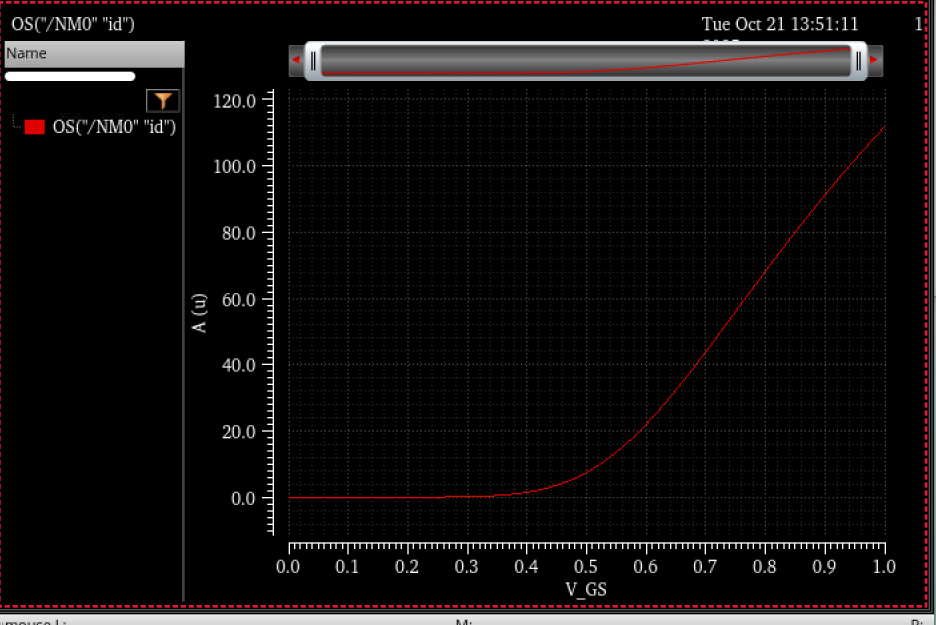
\includegraphics[width=0.8\textwidth]{image-43.png}
\caption{NMOS $I_D$ vs. $V_{GS}$特性曲线}
\label{fig:task1}
\end{figure}

\subsection{理论分析}
NMOS晶体管的$I_D$-$V_{GS}$特性曲线可以分为四个工作区域:

\textbf{1. 截止区:}当$V_{GS} < V_{TH}$时,晶体管处于截止状态,此时$I_D \approx 0$。从曲线可以看出,当$V_{GS}$较小时,漏极电流几乎为零。

\textbf{2. 亚阈值区:}当$V_{GS}$接近但小于$V_{TH}$时,晶体管进入亚阈值区,此时漏极电流呈指数增长:
\begin{equation}
I_D = I_0 e^{\frac{V_{GS}-V_{TH}}{nV_T}}
\end{equation}
其中$n$为亚阈值斜率因子,$V_T$为热电压(约26mV)。

\textbf{3. 饱和区:}当$V_{GS} > V_{TH}$时,晶体管进入强反型区。根据MOS晶体管的基本理论,在饱和区工作时:
\begin{equation}
I_D = \frac{1}{2}\mu_n C_{ox}\frac{W}{L}(V_{GS}-V_{TH})^2(1+\lambda V_{DS})
\end{equation}

\textbf{4. 线性区:}当$V_{GS}$继续增大,使得$V_{DS} < V_{GS} - V_{TH}$时,晶体管进入线性区。根据MOS晶体管的基本理论,在线性区工作时:
\begin{equation}
I_D = \frac{W}{L} \mu_n C_{ox}\left[(V_{GS}-V_{TH})V_{DS} - \frac{V_{DS}^2}{2}\right]
\end{equation}

从曲线形状可以看出:
\begin{itemize}
\item 在$V_{GS} < V_{TH}$时,电流几乎为零(截止区)
\item 在$V_{GS}$接近$V_{TH}$时,电流开始缓慢增加(亚阈值区)
\item 当$V_{GS} > V_{TH}$后,电流随$V_{GS}$呈近似二次方关系快速增长(强反型饱和区)
\item 随着$V_{GS}$进一步增大,电流增长速率减缓,近似呈线性增长(线性区)
\end{itemize}

\newpage
\section{任务二:跨导gm vs. VGS特性分析}

\subsection{任务要求}
\textbf{任务2:在报告中包含gm vs. VGS曲线,并根据理论分析为什么曲线是这样的形状。}

\subsection{实验结果}
图\ref{fig:task2}展示了NMOS晶体管的跨导$g_m$与栅源电压$V_{GS}$的关系曲线。

\begin{figure}[h]
\centering
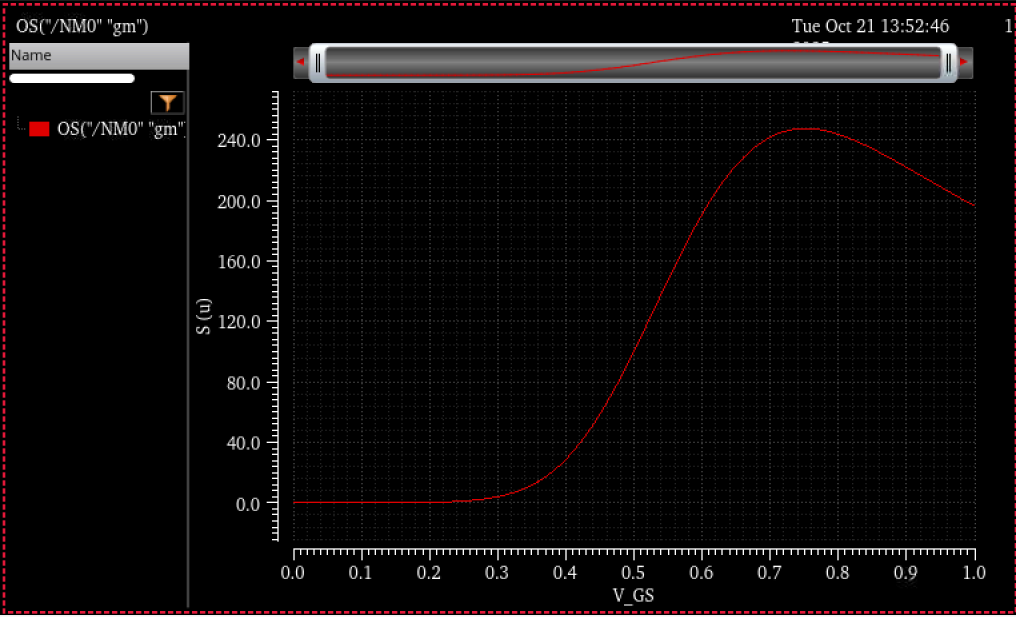
\includegraphics[width=0.8\textwidth]{image-44.png}
\caption{NMOS $g_m$ vs. $V_{GS}$特性曲线}
\label{fig:task2}
\end{figure}

\subsection{理论分析}
跨导$g_m$定义为漏极电流对栅源电压的偏导数:
\begin{equation}
g_m = \frac{\partial I_D}{\partial V_{GS}}
\end{equation}

根据任务一中的$I_D$表达式:
\begin{itemize}
  \item 在饱和区:
  \begin{equation}
  I_D = \frac{1}{2}\mu_n C_{ox}\frac{W}{L}(V_{GS}-V_{TH})^2(1+\lambda V_{DS})
  \end{equation}

  对$V_{GS}$求导可得:
  \begin{equation}
  g_m = \mu_n C_{ox}\frac{W}{L}(V_{GS}-V_{TH})(1+\lambda V_{DS})
  \end{equation}

  从理论公式可以看出,$g_m$与$(V_{GS}-V_{TH})$成线性关系。这与图\ref{fig:task2}中的曲线形状相符:

  \item 在线性区:
  \begin{equation}
  I_D = \frac{W}{L} \mu_n C_{ox}\left[(V_{GS}-V_{TH})V_{DS} - \frac{V_{DS}^2}{2}\right]
  \end{equation}

  对$V_{GS}$求导可得:
  \begin{equation}
  g_m = \mu_n C_{ox}\frac{W}{L}V_{DS}
  \end{equation}

  从理论公式可以看出,在线性区,$g_m$与$V_{DS}$成正比,与$V_{GS}$无关。这也与图\ref{fig:task2}中的曲线形状相符。

  \item 当$V_{GS}$进一步增大,栅控能力过强,导致沟道中的横向电场过大,出现速度饱和效应和非常迁移率效应,使得跨导增长速率减缓,甚至下降。
\end{itemize}

\newpage
\section{任务三:gm/ID特性分析与最佳工作点}

\subsection{任务要求}
\textbf{任务3:在报告中包含gm/id曲线,请分析最佳gm/id的工作点出现在什么区。这个区MOS能不能正常工作。能让MOS正常工作并能取得比较优异gm/id性能的工作区是哪个区。}

\subsection{实验结果}
图\ref{fig:task3}展示了NMOS晶体管的$g_m/I_D$与栅源电压$V_{GS}$的关系曲线。

\begin{figure}[h]
\centering
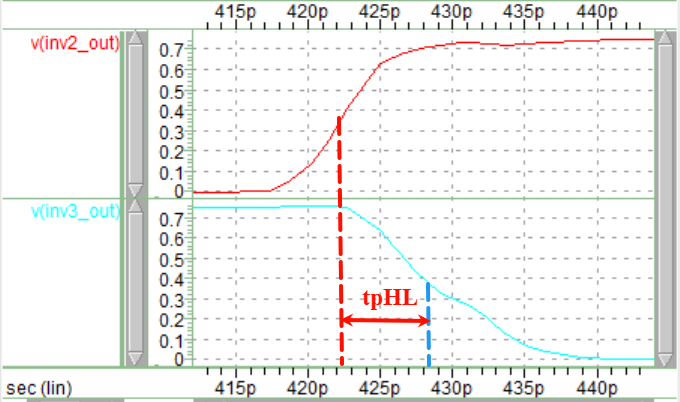
\includegraphics[width=0.8\textwidth]{image.png}
\caption{NMOS $g_m/I_D$ vs. $V_{GS}$特性曲线}
\label{fig:task3}
\end{figure}

\subsection{理论分析}
$g_m/I_D$比值是模拟集成电路设计中的一个重要参数,它反映了单位电流下晶体管的跨导效率,是衡量功耗效率的关键指标。

从理论分析可知,在不同工作区域:

\textbf{1. 亚阈值区:}
在亚阈值区,$I_D \propto e^{V_{GS}/nV_T}$,因此:
\begin{equation}
\frac{g_m}{I_D} = \frac{1}{nV_T} 
\end{equation}
此时$g_m/I_D$达到理论最大值。

\textbf{2. 弱反型到中等反型区:}
这是从亚阈值区过渡到强反型区的区域,$g_m/I_D$开始下降但仍保持较高水平。

\textbf{3. 强反型区(饱和区):}
在强反型饱和区:
\begin{equation}
\frac{g_m}{I_D} = \frac{2}{V_{GS}-V_{TH}}
\end{equation}
随着$V_{GS}$增加,$g_m/I_D$持续下降。

从图\ref{fig:task3}可以观察到:
\begin{itemize}
  \item 最佳$g_m/I_D$出现在\textbf{亚阈值区},此时$g_m/I_D$达到最大值

  然而,亚阈值区的工作电流极小,虽然功耗效率最高,但晶体管的驱动能力很弱,且速度很慢,不适合大多数模拟电路应用

  \item \textbf{中等反型区/饱和区}是最佳的折中工作区域,这个区域的$g_m/I_D$仍然较高,同时有足够的电流驱动能力和合理的工作速度
\end{itemize}

\newpage
\section{任务四:ID vs. VGS and VDS三维特性分析}

\subsection{任务要求}
\textbf{任务4:在报告中包含ID vs. VGS and VDS曲线,并简要解释该曲线特性。}

\subsection{实验结果}
图\ref{fig:task4a}和图\ref{fig:task4b}分别展示了漏极电流$I_D$随栅源电压$V_{GS}$和漏源电压$V_{DS}$变化的三维特性曲线。

\begin{figure}[h]
\centering
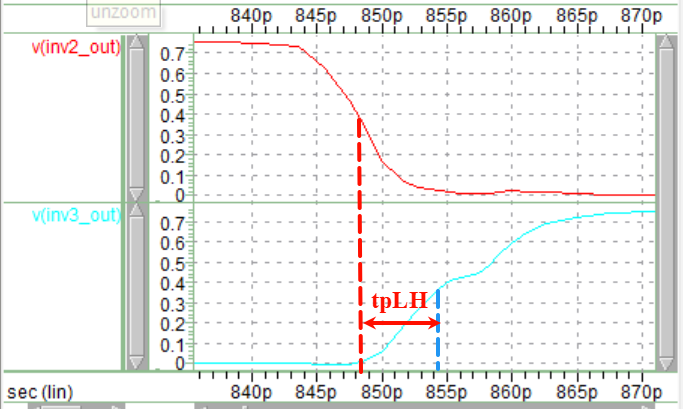
\includegraphics[width=0.8\textwidth]{image-1.png}
\caption{NMOS $I_D$ vs. $V_{GS}$ 特性曲线}
\label{fig:task4a}
\end{figure}

\begin{figure}[h]
\centering
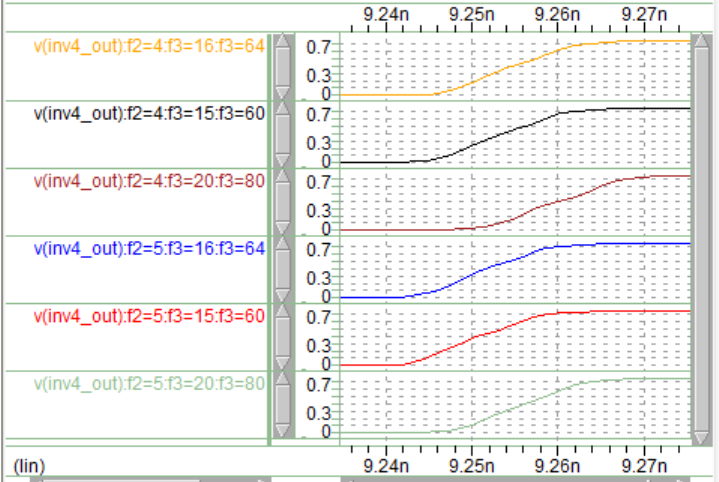
\includegraphics[width=0.8\textwidth]{image-2.png}
\caption{NMOS $I_D$ vs.$V_{DS}$特性曲线}
\label{fig:task4b}
\end{figure}

\subsection{理论分析}
NMOS晶体管的完整工作特性由$I_D$、$V_{GS}$和$V_{DS}$三个参数共同决定。根据MOS晶体管理论,可以将工作区域分为:

\textbf{1. 截止区:}
当$V_{GS} < V_{TH}$时,无论$V_{DS}$取何值,$I_D \approx 0$。例如图\ref{fig:task4a}和图\ref{fig:task4b}中,当$V_{GS}$较低时,曲线簇接近零。

\textbf{2. 线性区:}
当$V_{GS} > V_{TH}$且$V_{DS} < V_{GS}-V_{TH}$时:
\begin{equation}
I_D = \mu_n C_{ox}\frac{W}{L}\left[(V_{GS}-V_{TH})V_{DS} - \frac{V_{DS}^2}{2}\right]
\end{equation}
此时$I_D$近似与$V_{DS}$成线性关系。从图\ref{fig:task4b}中可以看到,在低$V_{DS}$区域,曲线簇随$V_{DS}$线性上升。

\textbf{3. 饱和区:}
当$V_{GS} > V_{TH}$且$V_{DS} \geq V_{GS}-V_{TH}$时:
\begin{equation}
I_D = \frac{1}{2}\mu_n C_{ox}\frac{W}{L}(V_{GS}-V_{TH})^2(1+\lambda V_{DS})
\end{equation}
此时$I_D$主要由$V_{GS}$控制,对$V_{DS}$的依赖性较弱(沟道长度调制效应)。这一点在图\ref{fig:task4b}中可以观察到,在高$V_{DS}$区域,曲线簇趋于平坦。



\newpage
\section{任务五:NMOS关键参数提取与计算}

\subsection{任务要求}
\textbf{任务5:在报告中包含$\mu C_{ox}$、$|V_{th}|$、$\lambda$计算过程和结果。}

\subsection{实验数据与计算过程}
\subsubsection{输出电阻$r_o$的提取}
在$V_{GS}=800$mV时,选取两个工作点(图\ref{fig:task5a}):
\begin{itemize}
\item 点1:$(V_{DS}, I_D) = (526.32\text{mV}, 87.396\mu\text{A})$
\item 点2:$(V_{DS}, I_D) = (810.74\text{mV}, 98.78\mu\text{A})$
\end{itemize}

从而得到:
\begin{equation}
  r_o = \frac{\Delta V_{DS}}{\Delta I_D} = \frac{810.74\text{mV}-526.32\text{mV}}{98.78\mu\text{A}-87.396\mu\text{A}} = 24950.9\Omega
\end{equation}
\begin{figure}[h]
\centering
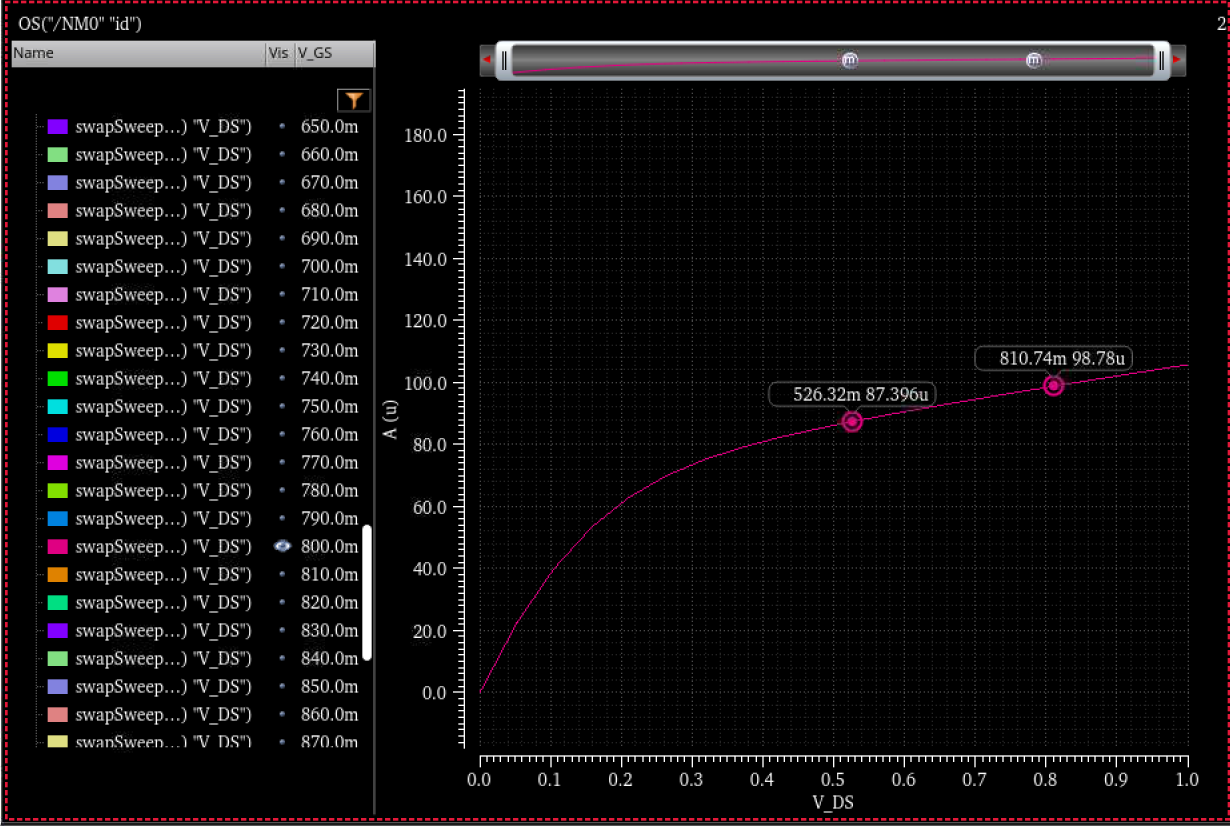
\includegraphics[width=0.8\textwidth]{image-3.png}
\caption{阈值电压测量点选取}
\label{fig:task5a}
\end{figure}


\subsubsection{阈值电压$V_{th}$的提取}

通过将NMOS偏置在$V_{GS}=800\text{mV}$, $V_{DS}=600\text{mV}$时,得到(图\ref{fig:task5b}):
\begin{equation}
V_{th} = 308.096\text{ mV}
\end{equation}

\begin{figure}[h]
\centering
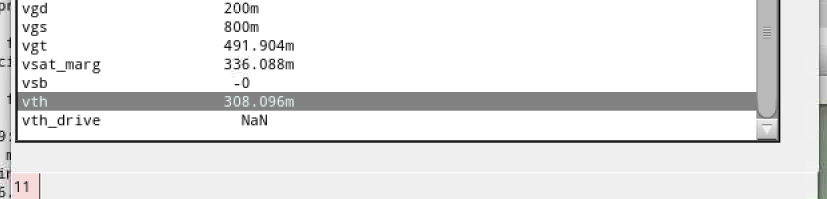
\includegraphics[width=0.6\textwidth]{image-7.png}
\caption{阈值电压$V_{th}$计算结果}
\label{fig:task5b}
\end{figure}

\subsubsection{沟道长度调制参数$\lambda$的提取}

输出电阻$r_o=24950.9\Omega$

通过将NMOS偏置在$V_{GS}=800\text{mV}$, $V_{DS}=600\text{mV}$时,得到(图\ref{fig:task5d}):
$I_{DS}=90.57\mu A$

\begin{figure}[h]
\centering
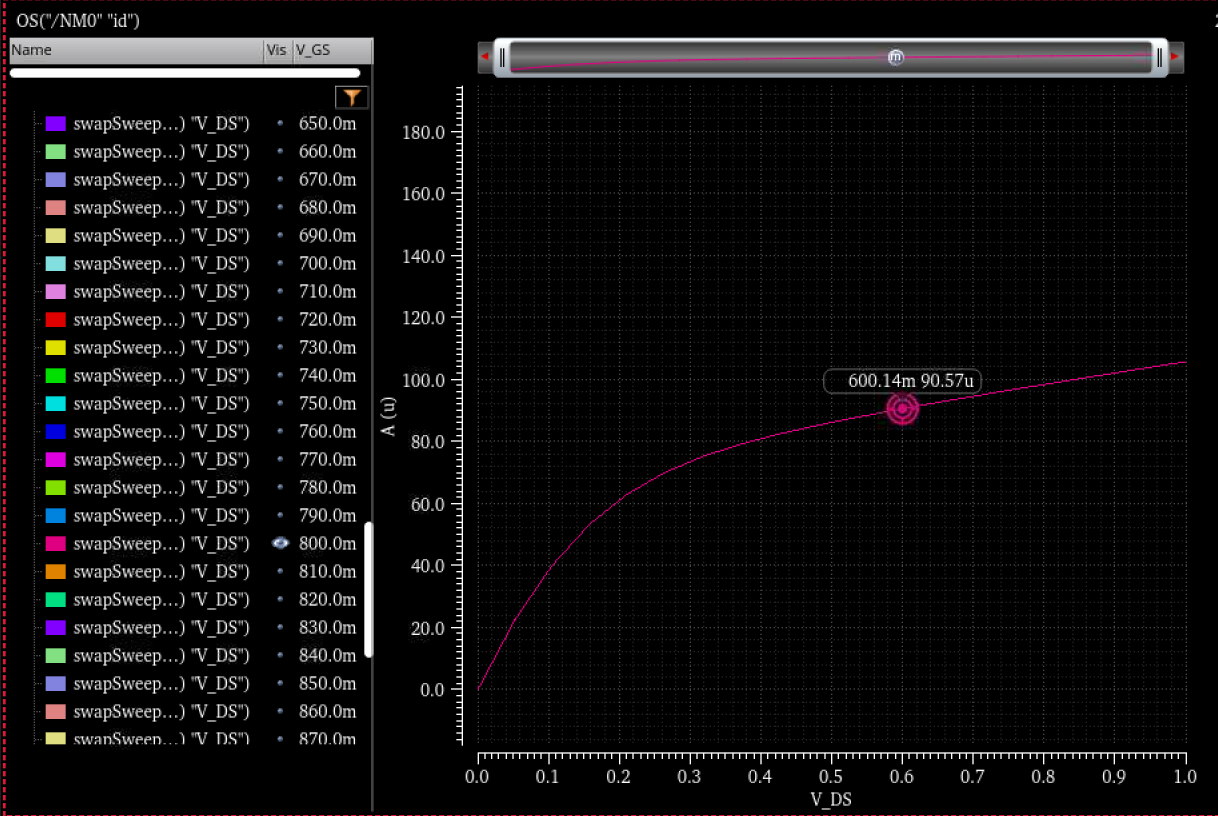
\includegraphics[width=0.6\textwidth]{image-5.png}
\caption{$V_{GS}=800\text{mV}$, $V_{DS}=600.14\text{mV}$时的$I_{DS}$}
\label{fig:task5d}
\end{figure}

最终得到:
\begin{equation}
\lambda = \frac{1}{r_o I_{DS}} = \frac{1}{24950.9\Omega \times 90.57\mu A} = 0.4423\text{ V}^{-1}
\end{equation}

\subsubsection{迁移率与栅氧化层电容乘积$\mu C_{ox}$的提取}

使用以下工作点参数:
\begin{itemize}
\item $W = 500$nm
\item $L = 60$nm
\item $I_D = 90.57\mu$A
\item $V_{GS} = 800$mV
\item $V_{DS} = 600.14$mV
\item $V_{TH} = 308.096$mV
\end{itemize}

根据饱和区电流公式:
\begin{equation}
I_D = \frac{1}{2}\mu C_{ox}\frac{W}{L}(V_{GS}-V_{TH})^2(1+\lambda V_{DS})
\end{equation}

可以求解:
\begin{equation}
\mu C_{ox} = \frac{2I_D}{(W/L)(V_{GS}-V_{TH})^2(1+\lambda V_{DS})} 
\end{equation}
代入数值后,计算得到:
\begin{equation}
\mu C_{ox} \approx 7.10 \times 10^{-5}\text{ A/V}^2
\end{equation}

\subsubsection{输出电阻$r_o$的另一种计算方法}

输出电阻也可以通过输出电导$g_{ds}$来计算:
\begin{equation}
r_o = \frac{1}{g_{ds}}
\end{equation}

其中$g_{ds} = \frac{\partial I_D}{\partial V_{DS}}$。图\ref{fig:task5h}通过NMOS的DC工作点获取直接得到了$g_{ds}$的值:$g_{ds} = 42.2342\mu\text{S}$

\begin{figure}[h]
\centering
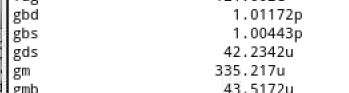
\includegraphics[width=0.7\textwidth]{image-10.png}
\caption{$g_{ds}$测量结果}
\label{fig:task5h}
\end{figure}

因此:
\begin{equation}
r_o = \frac{1}{g_{ds}} = \frac{1}{42.2342\mu\text{S}} = 23677.493\Omega
\end{equation}

\subsection{理论分析}
以上三个参数是MOSFET建模的关键参数:

\textbf{1. 阈值电压$V_{th}$:}决定了晶体管的开启电压,是工艺和器件设计的重要参数。

\textbf{2. 沟道长度调制参数$\lambda$:}描述了饱和区输出电流对$V_{DS}$的依赖性。$\lambda$越大,表示沟道长度调制效应越明显,输出电阻$r_o$越小。从计算结果看,$\lambda = 0.4423$ V$^{-1}$表示该短沟道器件的沟道长度调制效应比较明显。

\textbf{3. $\mu C_{ox}$:}反映了器件的工艺参数,决定了晶体管的电流驱动能力。对于给定的工艺,$\mu C_{ox}$是一个常数。

\newpage
\section{任务六:输出电阻ro的分析}

\subsection{任务要求}
\textbf{在报告中包含ro的计算过程和结果图,并简要分析。}

\subsection{实验结果}
图\ref{fig:task6a}和图\ref{fig:task6b}展示了输出电阻$r_o$随工作条件变化的特性。

\begin{figure}[h]
\centering
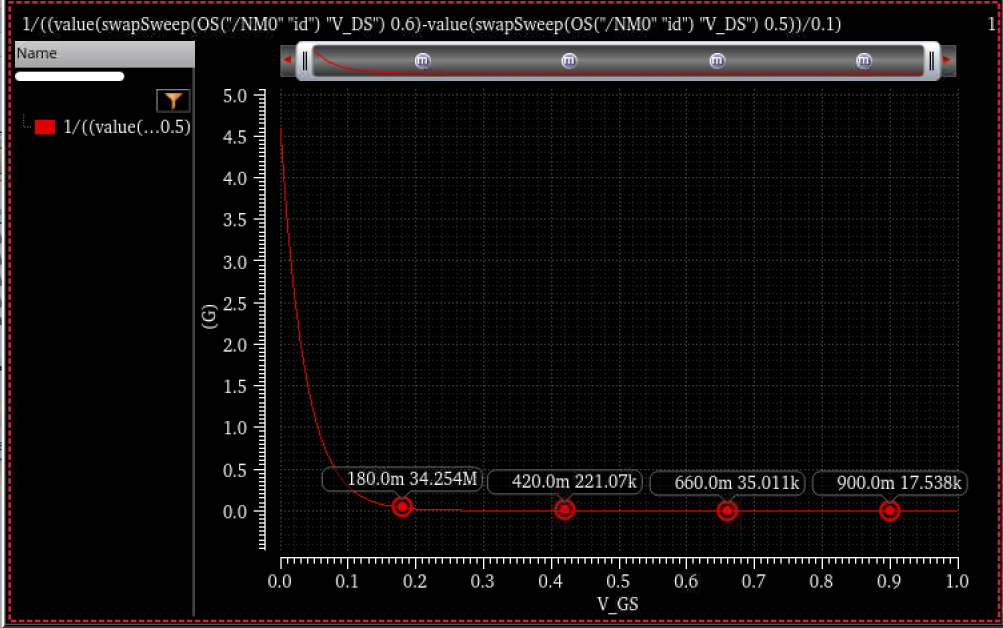
\includegraphics[width=0.8\textwidth]{image-12.png}
\caption{输出电阻$r_o$特性曲线(图1)}
\label{fig:task6a}
\end{figure}

\begin{figure}[h]
\centering
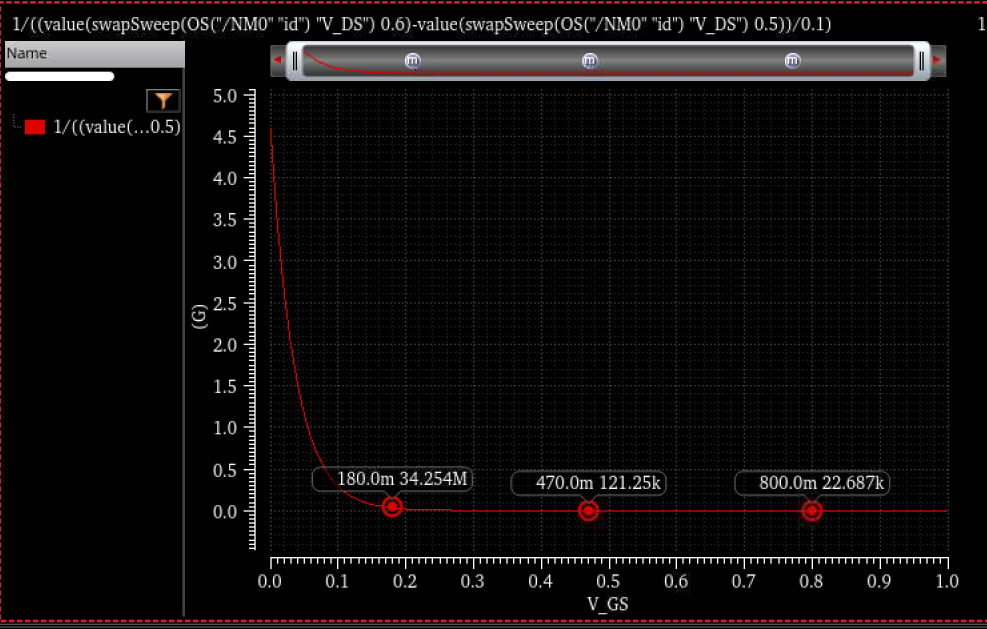
\includegraphics[width=0.8\textwidth]{image-13.png}
\caption{输出电阻$r_o$特性曲线(图2)}
\label{fig:task6b}
\end{figure}

\subsection{理论分析}
输出电阻$r_o$定义为:
\begin{equation}
r_o = \frac{\partial V_{DS}}{\partial I_D}\bigg|_{V_{GS}=\text{const}}
\end{equation}

在饱和区,考虑沟道长度调制效应:
\begin{equation}
r_o = \frac{1}{\lambda I_D}
\end{equation}

从理论公式可以看出:
\begin{itemize}
\item $r_o$与漏极电流$I_D$成反比关系
\item $r_o$与沟道长度调制参数$\lambda$成反比关系
\end{itemize}

从图\ref{fig:task6a}和图\ref{fig:task6b}可以观察到:
\begin{itemize}
\item 随着$V_{GS}$增加,$I_D$增大,因此$r_o$减小
\item 在低电流区域,$r_o$很大,输出特性接近理想电流源
\item 在高电流区域,$r_o$变小,沟道长度调制效应更加明显
\end{itemize}

\newpage
\section{任务七:本征增益与尺寸优化分析}
\subsection{任务要求}
\textbf{扫描MOS尺寸,观察本征增益与尺寸和VDS的关系。请找出最大本征增益对应的偏置条件与尺寸。并尝试用理论解释。}

\subsection{实验结果}

\subsubsection{gm/id性能优化}

仿真命令设置如图\ref{fig:task7a}所示:
\begin{figure}[h]
\centering
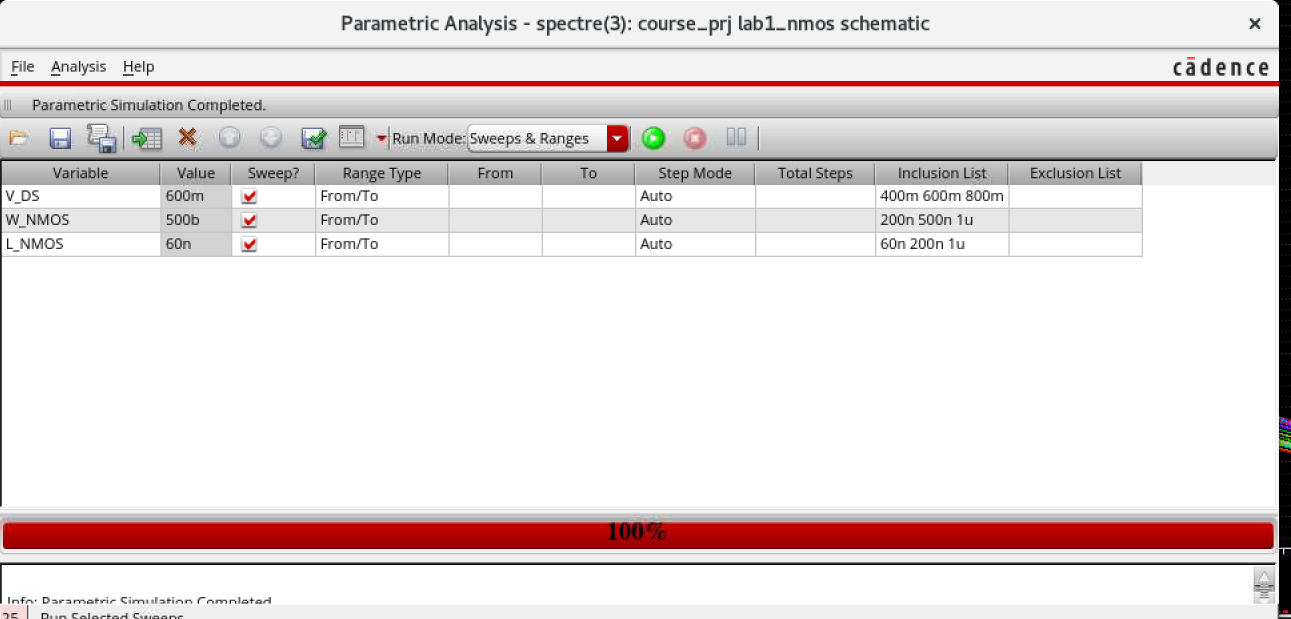
\includegraphics[width=0.7\textwidth]{image-15.png}
\caption{仿真命令设置}
\label{fig:task7a}
\end{figure}

仿真结果如图\ref{fig:task7b}所示。可以看出,当$V_{DS}=400$mV,$W=1\mu m, L=200nm$时,$g_m/I_D$在整体$V_{GS}$范围内达到了最大值。原因为:当$W$较大,$L$较小,$V_{DS}$较低时,器件工作在中等反型区,既保证了较高的$g_m$,又有足够的电流驱动能力($I_{DS}$)。

\begin{figure}[h]
\centering
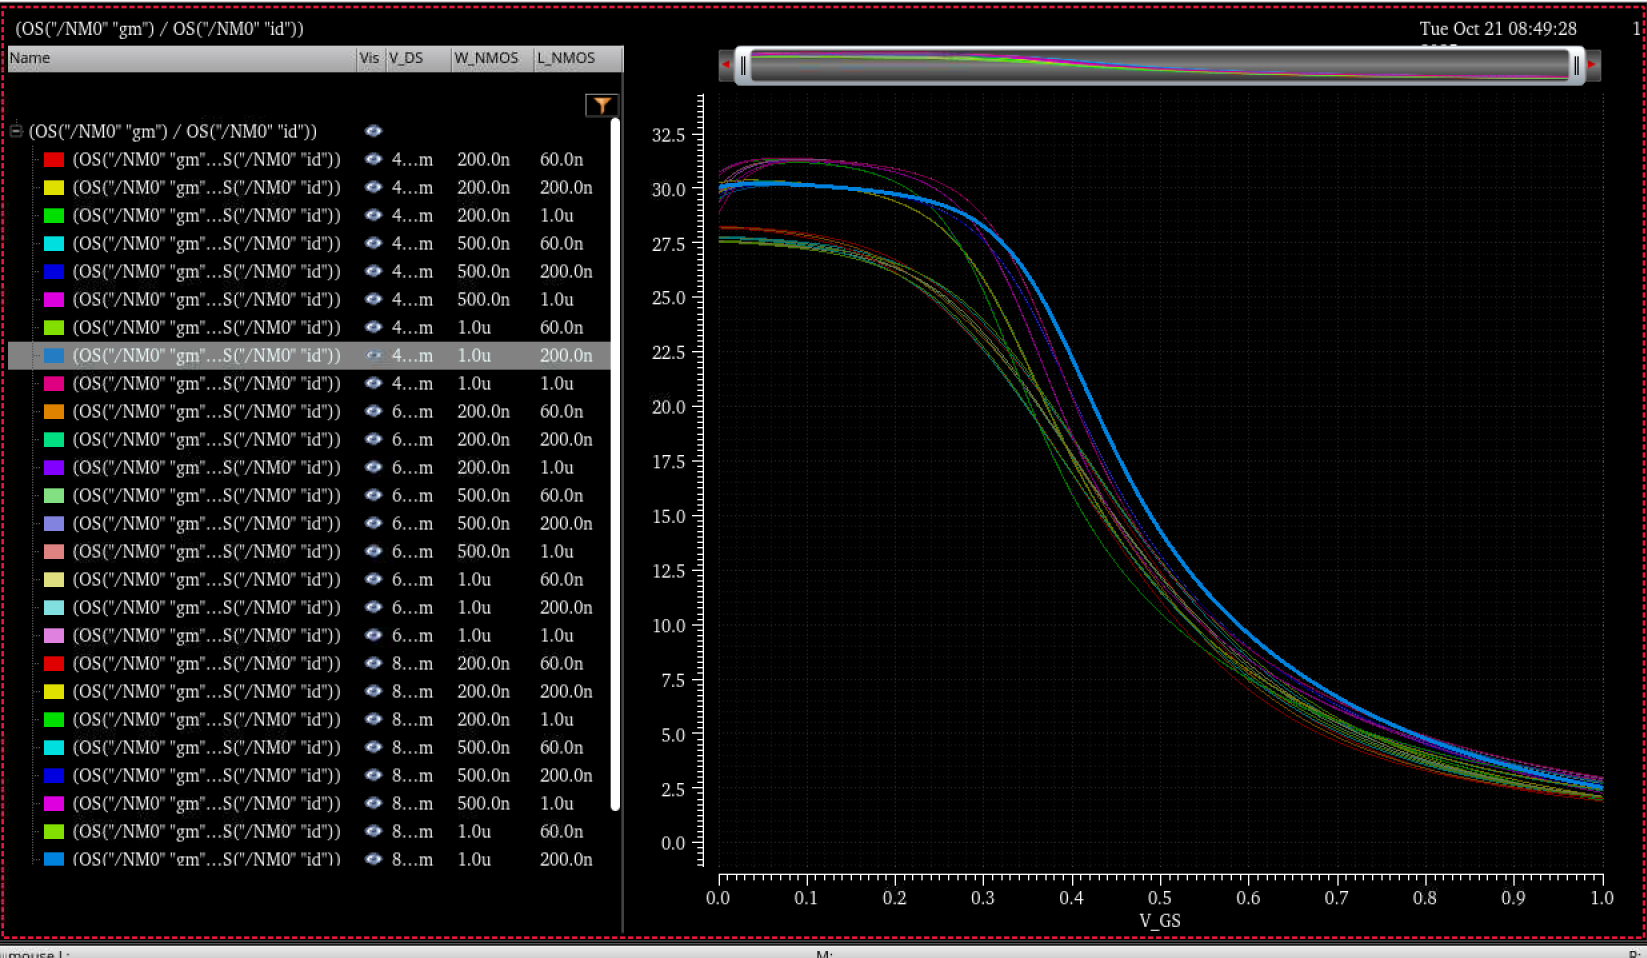
\includegraphics[width=0.8\textwidth]{image-14.png}
\caption{$g_m/I_D$性能测试结果}
\label{fig:task7b}
\end{figure}


\subsubsection{本征增益分析}
首先在$W=500$nm,$L=60$nm条件下测试本征增益与$V_{DS}$的关系,结果如图\ref{fig:task7c}所示:

\begin{figure}[h]
\centering
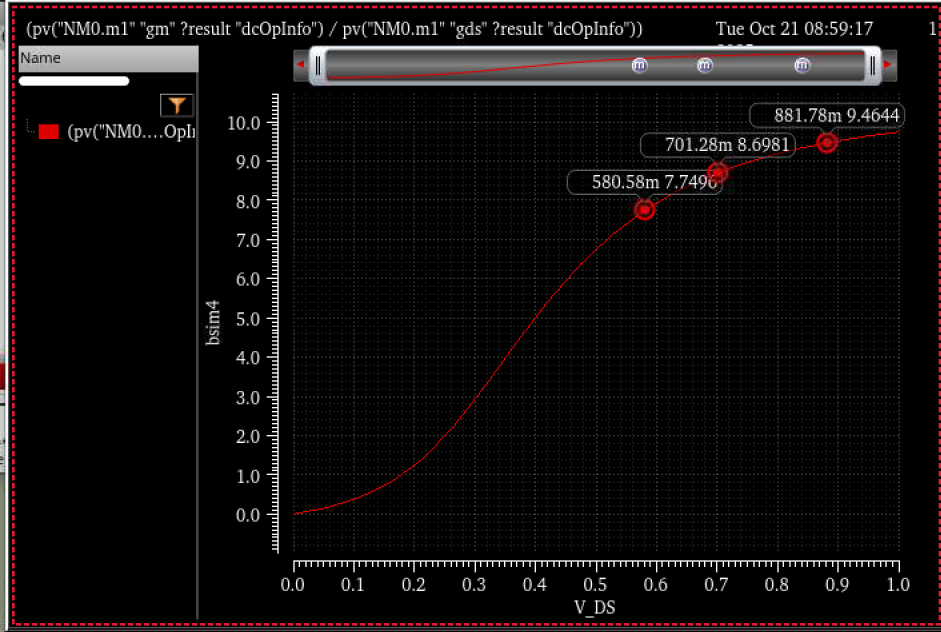
\includegraphics[width=0.8\textwidth]{image-16.png}
\caption{本征增益vs. $V_{DS}$($W=500$nm, $L=60$nm)}
\label{fig:task7c}
\end{figure}

然后进行参数扫描,扫描参数设置如图\ref{fig:task7d}所示:

\begin{figure}[h]
\centering
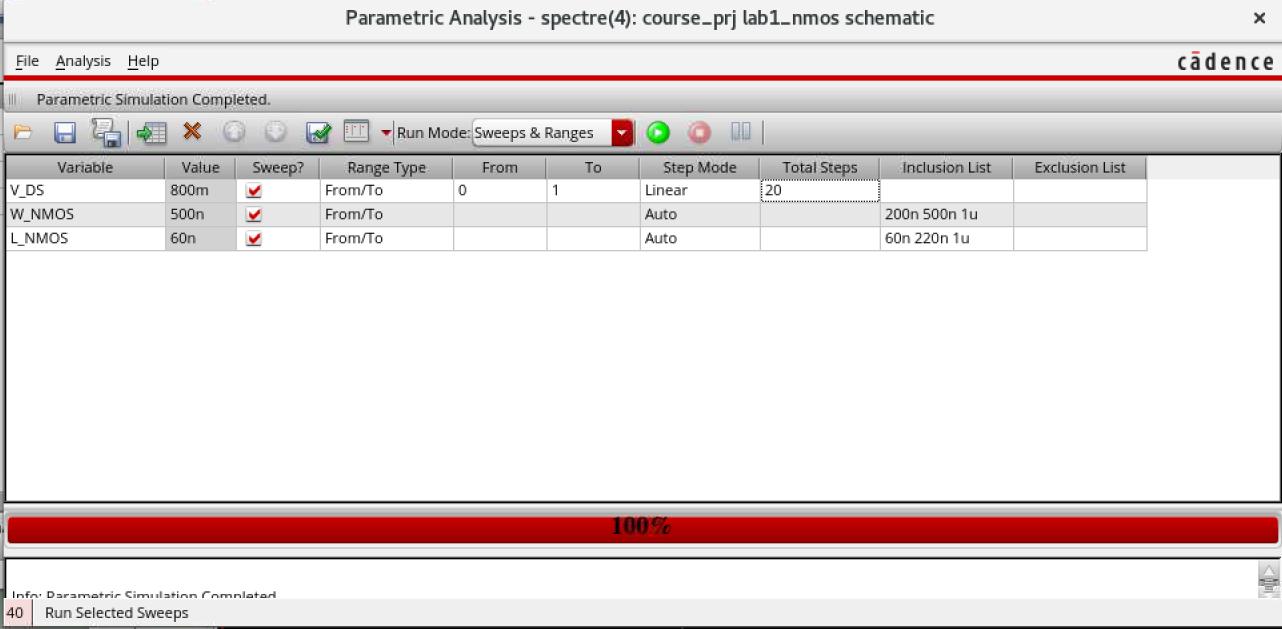
\includegraphics[width=0.7\textwidth]{image-18.png}
\caption{本征增益扫描参数设置}
\label{fig:task7d}
\end{figure}

扫描结果如图\ref{fig:task7e}所示。可知,在$W$, $L$均为设置的最大值:$1\mu m$时,本征增益达到了最大值。

\begin{figure}[h]
\centering
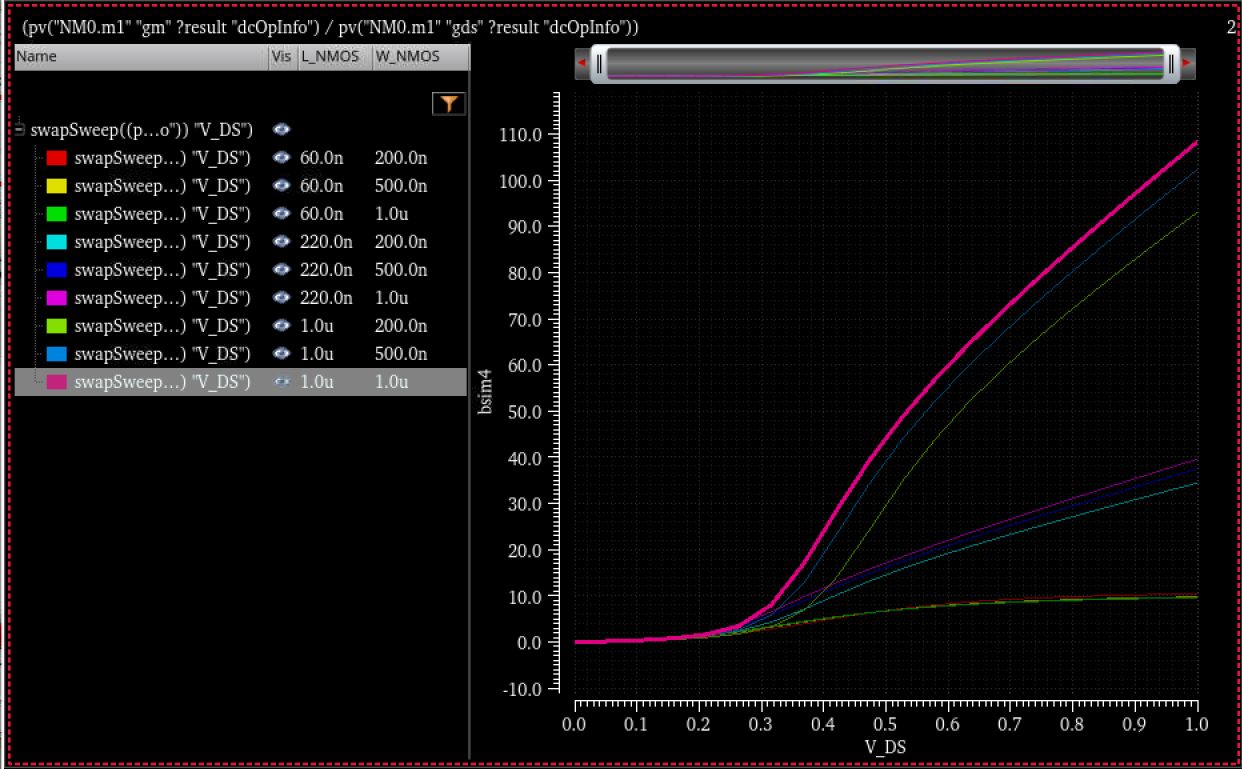
\includegraphics[width=0.8\textwidth]{image-17.png}
\caption{本征增益参数扫描结果}
\label{fig:task7e}
\end{figure}

\subsection{理论分析}
本征增益(Intrinsic Gain)定义为:
\begin{equation}
A_0 = g_m \cdot r_o
\end{equation}

这是单个MOSFET能够实现的最大电压增益。

\subsubsection{本征增益的理论推导}
在饱和区:
\begin{equation}
g_m = \sqrt{2\mu C_{ox}\frac{W}{L}I_D}
\end{equation}

\begin{equation}
r_o = \frac{1}{\lambda I_D}
\end{equation}

因此本征增益为:
\begin{equation}
A_0 = g_m \cdot r_o = \frac{\sqrt{2\mu C_{ox}\frac{W}{L}I_D}}{\lambda I_D} = \frac{1}{\lambda}\sqrt{\frac{2\mu C_{ox}(W/L)}{I_D}}
\end{equation}

也可以写成:
\begin{equation}
A_0 = \frac{2}{\lambda(V_{GS}-V_{TH})}
\end{equation}

从理论分析可以得出:
\begin{itemize}
\item 尺寸选择上:

增加沟道长度$L$可以减小$\lambda$,从而增大$A_0$

当沟道宽度$W$增大时,$g_m$增大,但$I_D$也增大,如果是长沟道器件,我们可以认为电流饱和,$I_D$不再增大,此时我们可以认为$A_0$增大。

\item 偏置条件上:

在较低的过驱动电压$(V_{GS}-V_{TH})$下工作可以获得更高的$A_0$
\end{itemize}


\newpage
\section{任务八:CMOS反相器DC特性分析}

\subsection{任务要求}
\textbf{任务8:在报告中包含该DC扫描的结果,并简要分析输入输出关系。}

\subsection{实验结果}
图\ref{fig:task8}展示了CMOS反相器的DC传输特性曲线(电压传输特性,VTC)。

\begin{figure}[h]
\centering
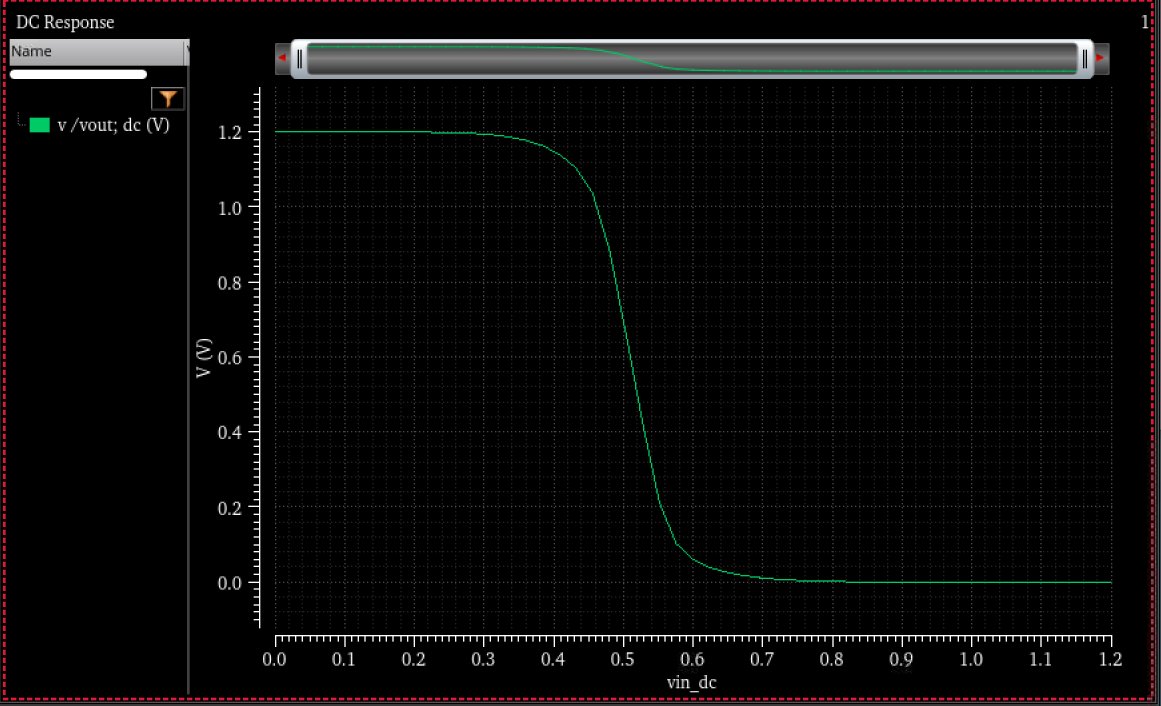
\includegraphics[width=0.8\textwidth]{image-19.png}
\caption{CMOS反相器DC传输特性}
\label{fig:task8}
\end{figure}

\subsection{理论分析}
CMOS反相器是最基本的数字逻辑门,也是模拟电路中常用的放大器结构。其DC传输特性可以分为五个工作区域:

\textbf{区域I:$V_{in}$很低(接近0V)}
\begin{itemize}
\item NMOS截止,PMOS导通并工作在线性区
\item $V_{out} \approx V_{DD}$(逻辑高电平)
\end{itemize}

\textbf{区域II:$V_{in}$增加至NMOS开启}
\begin{itemize}
\item NMOS进入饱和区,PMOS仍在线性区
\item $V_{out}$开始下降,但下降缓慢
\end{itemize}

\textbf{区域III:转换区(两管都在饱和区)}
\begin{itemize}
\item NMOS和PMOS都工作在饱和区
\item 此时增益最大:$A_v = -(g_{mn} + g_{mp})/(g_{dsn} + g_{dsp})$
\item $V_{out}$随$V_{in}$快速下降,曲线斜率最大
\end{itemize}

\textbf{区域IV:$V_{in}$继续增加}
\begin{itemize}
\item NMOS在线性区,PMOS在饱和区
\item $V_{out}$继续下降但速度减慢
\end{itemize}

\textbf{区域V:$V_{in}$接近$V_{DD}$}
\begin{itemize}
\item NMOS在线性区完全导通,PMOS截止
\item $V_{out} \approx 0$V(逻辑低电平)
\end{itemize}




\newpage
\section{任务九:CMOS反相器尺寸优化}

\subsection{任务要求}
\textbf{任务9:在报告中记录修改结果,并尝试理论分析或者公式求解。}

\subsection{实验结果}

\subsubsection{PMOS宽度优化}
通过二分法搜索最佳PMOS宽度,使得输出电压$V_{out} \approx 600$mV(接近$V_{DD}/2$):

\begin{itemize}
\item $W_P = 2\mu$m:$V_{out} = 112.304$mV(图\ref{fig:task9a})
\item $W_P = 4\mu$m:$V_{out} = 988.216$mV(图\ref{fig:task9b})
\item $W_P = 3\mu$m:$V_{out} = 519.076$mV(图\ref{fig:task9c})
\item $W_P = 3.5\mu$m:$V_{out} = 795.958$mV(图\ref{fig:task9d})
\item $W_P = 3.25\mu$m:$V_{out} = 664.743$mV(图\ref{fig:task9e})
\item $W_P = 3.125\mu$m:$V_{out} = 593.273$mV(图\ref{fig:task9f})
\item $W_P = 3.15\mu$m:$V_{out} = 907.824$mV(图\ref{fig:task9g})
\item $W_P = 3.135\mu$m:$V_{out} = 599.109$mV(图\ref{fig:task9h})
\end{itemize}

最终选择$W_P = 3.13\mu$m。

\begin{figure}[htbp]
    \centering
    % 第一张子图
    \begin{subfigure}[b]{0.45\textwidth} % 子图宽度为总宽度的45%
        \centering
        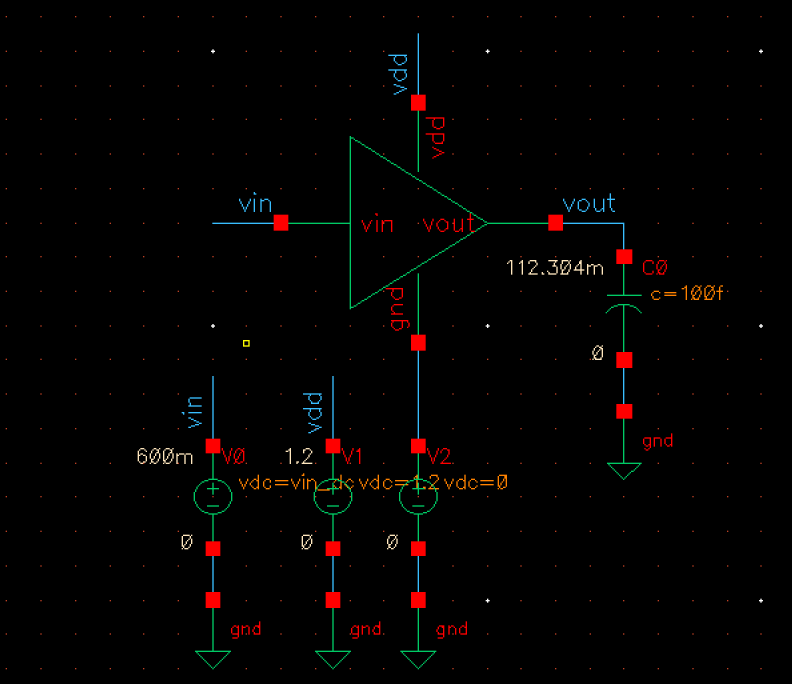
\includegraphics[width=\textwidth]{image-20.png} 
        \caption{$W_P = 2\mu$m,$V_{out} = 112.304$mV}
        \label{fig:task9a}
    \end{subfigure}
    \hfill % 添加水平间距
    % 第二张子图
    \begin{subfigure}[b]{0.45\textwidth}
        \centering
        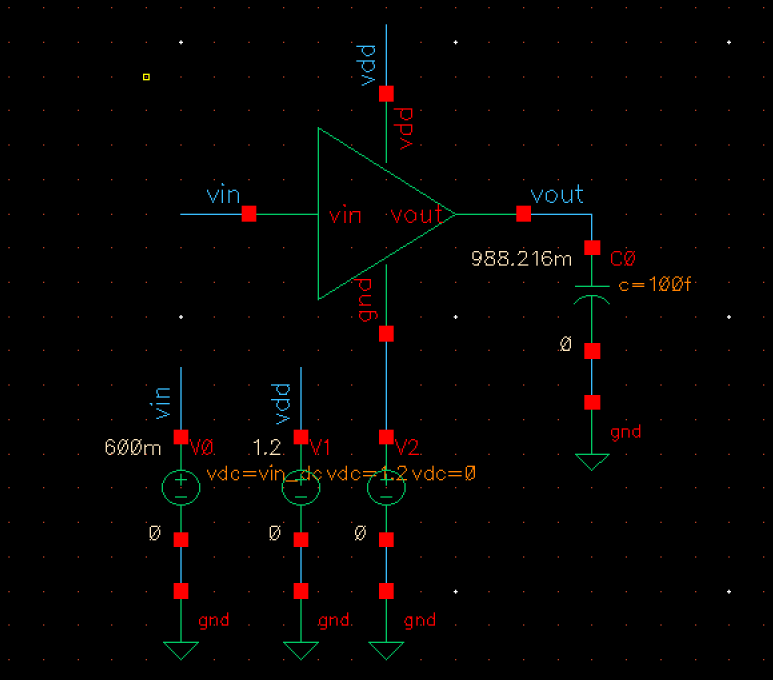
\includegraphics[width=\textwidth]{image-21.png} 
        \caption{$W_P = 4\mu$m,$V_{out} = 988.216$mV}
        \label{fig:task9b}
    \end{subfigure}
    \label{fig:task9ab}
    % 总图标题
    \caption{二分法第一组}
\end{figure}

\begin{figure}[htbp]
    \centering
    % 第一张子图
    \begin{subfigure}[b]{0.45\textwidth} % 子图宽度为总宽度的45%
        \centering
        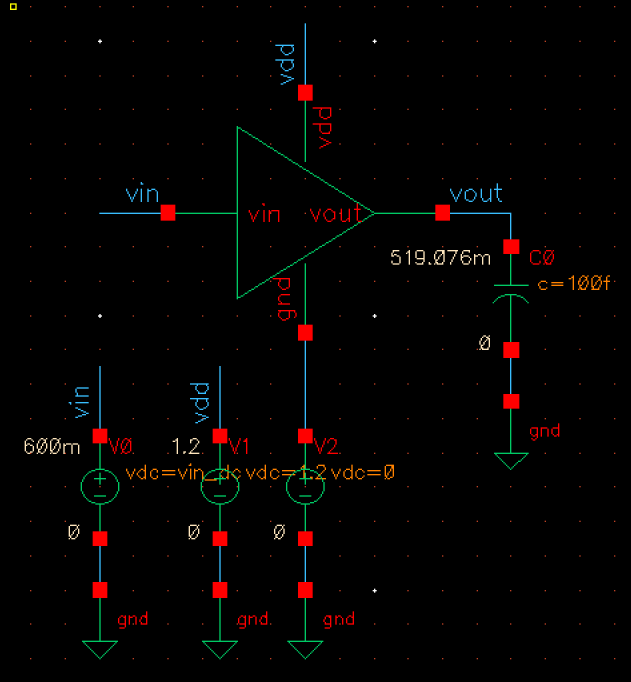
\includegraphics[width=\textwidth]{image-22.png} 
        \caption{$W_P = 3\mu$m,$V_{out} = 519.076$mV}
        \label{fig:task9c}
    \end{subfigure}
    \hfill % 添加水平间距
    % 第二张子图
    \begin{subfigure}[b]{0.45\textwidth}
        \centering
        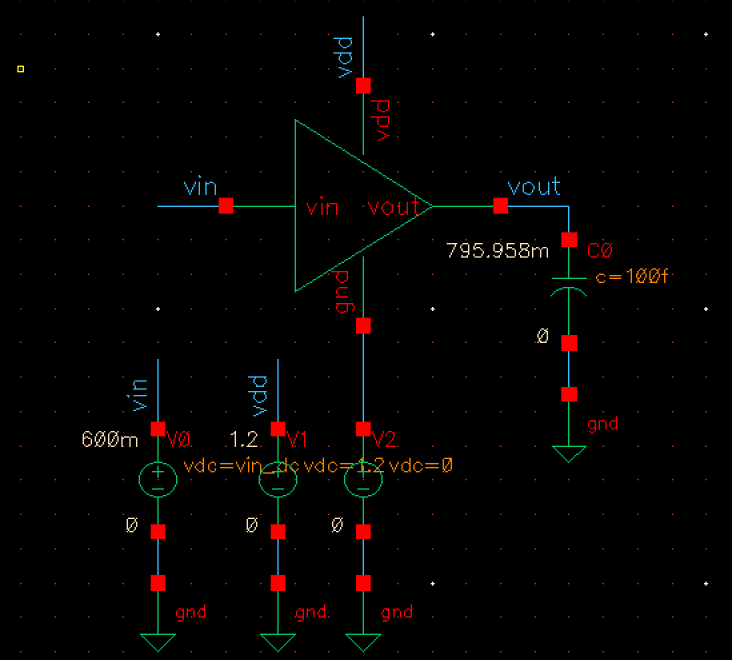
\includegraphics[width=\textwidth]{image-23.png} 
        \caption{$W_P = 3.5\mu$m,$V_{out} = 795.958$mV}
        \label{fig:task9d}
    \end{subfigure}
    % 总图标题
    \label{fig:task9cd}
    \caption{二分法第二组}
\end{figure}

\begin{figure}[htbp]
    \centering
    % 第一张子图
    \begin{subfigure}[b]{0.45\textwidth} % 子图宽度为总宽度的45%
        \centering
        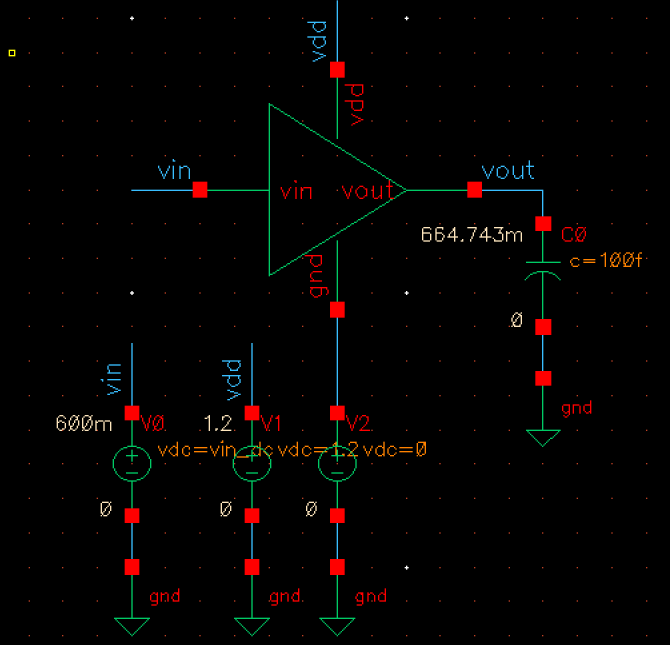
\includegraphics[width=\textwidth]{image-24.png} 
        \caption{$W_P = 3.25\mu$m,$V_{out} = 664.743$mV}
        \label{fig:task9e}
    \end{subfigure}
    \hfill % 添加水平间距
    % 第二张子图
    \begin{subfigure}[b]{0.45\textwidth}
        \centering
        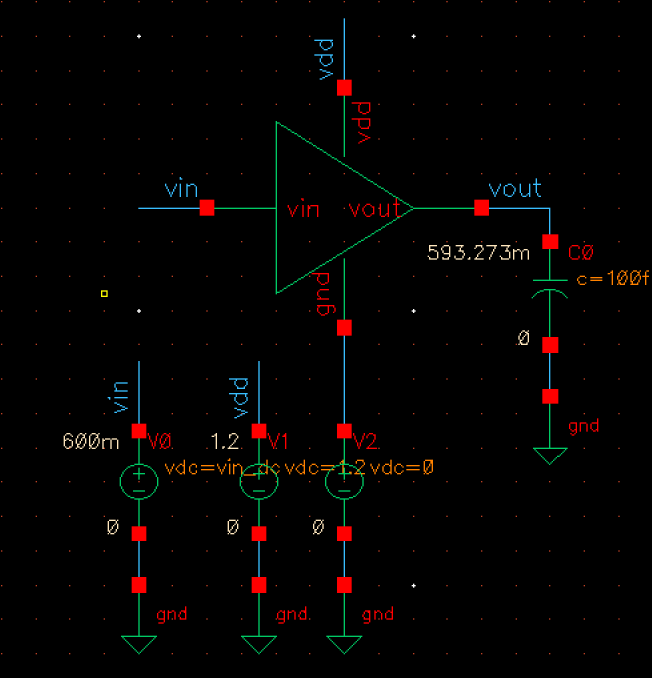
\includegraphics[width=\textwidth]{image-26.png} 
        \caption{$W_P = 3.125\mu$m,$V_{out} = 593.273$mV}
        \label{fig:task9f}
    \end{subfigure}
    % 总图标题
    \label{fig:task9ef}
    \caption{二分法第三组}
\end{figure}

\begin{figure}[htbp]
    \centering
    % 第一张子图
    \begin{subfigure}[b]{0.45\textwidth} % 子图宽度为总宽度的45%
        \centering
        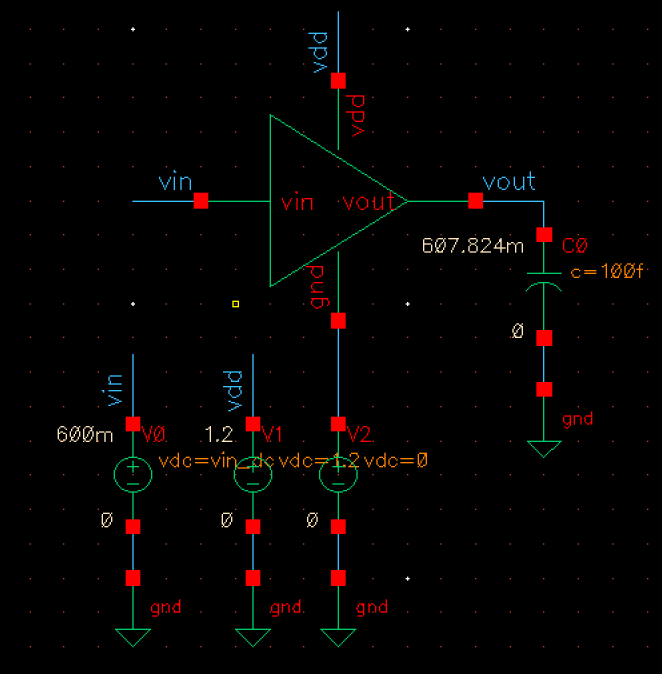
\includegraphics[width=\textwidth]{image-27.png} 
        \caption{$W_P = 3.15\mu$m,$V_{out} = 607.824$mV}
        \label{fig:task9g}
    \end{subfigure}
    \hfill % 添加水平间距
    % 第二张子图
    \begin{subfigure}[b]{0.45\textwidth}
        \centering
        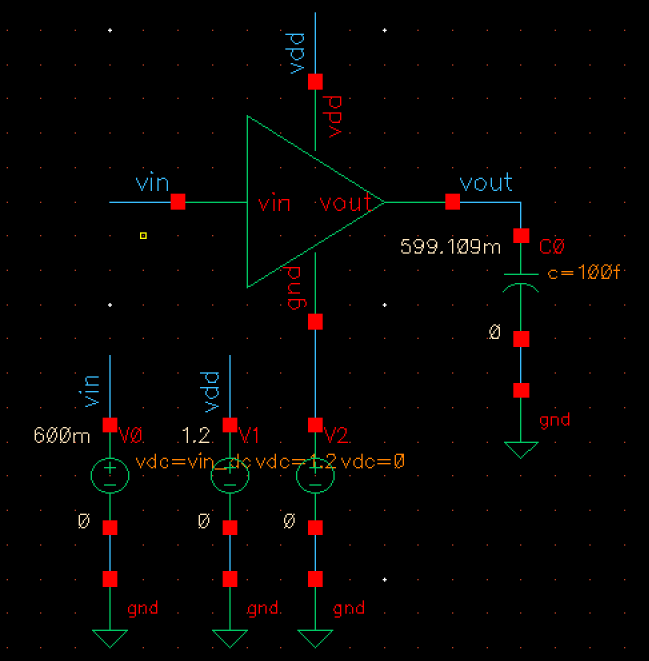
\includegraphics[width=\textwidth]{image-28.png} 
        \caption{$W_P = 3.135\mu$m,$V_{out} = 599.109$mV}
        \label{fig:task9h}
    \end{subfigure}
    % 总图标题
    \label{fig:task9gh}
    \caption{二分法第四组}
\end{figure}


\subsubsection{Finger数量影响分析}
固定总宽度$W_P = 3.13\mu$m,改变finger数量和单个finger宽度:

\begin{itemize}
\item Fingers = 1,Finger Width = $3.13\mu$m(图\ref{fig:task9i})
\item Fingers = 2,Finger Width = $1.565\mu$m(图\ref{fig:task9j})
\item Fingers = 3,Finger Width = $1.045\mu$m(图\ref{fig:task9k})
\item Fingers = 4,Finger Width = $780$nm(图\ref{fig:task9l})
\item Fingers = 5,Finger Width = $625$nm(图\ref{fig:task9m})
\end{itemize}

\begin{figure}[htbp]
    \centering
    % 第一张子图
    \begin{subfigure}[b]{0.45\textwidth} % 子图宽度为总宽度的45%
        \centering
        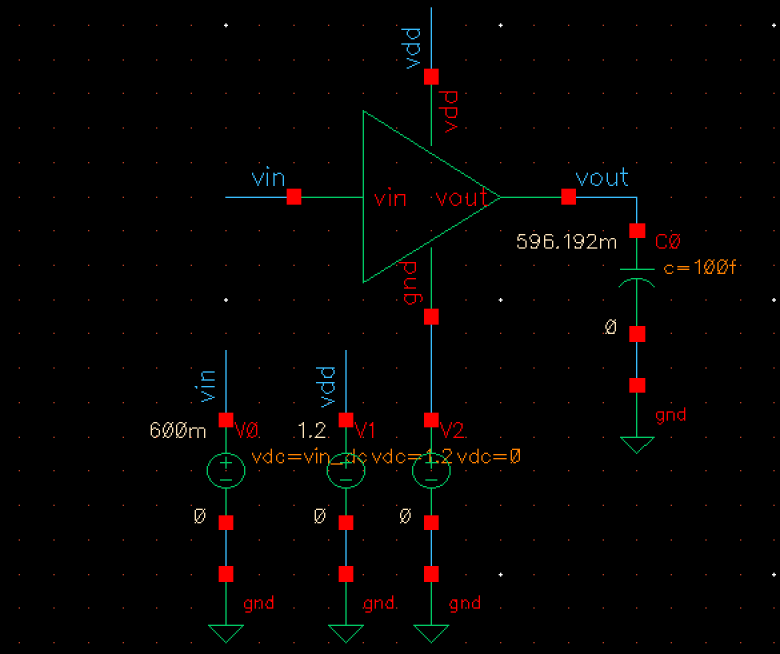
\includegraphics[width=\textwidth]{image-30.png} 
        \caption{Fingers = 1,Finger Width = $3.13\mu$m}
        \label{fig:task9i}
    \end{subfigure}
    \hfill % 添加水平间距
    % 第二张子图
    \begin{subfigure}[b]{0.45\textwidth}
        \centering
        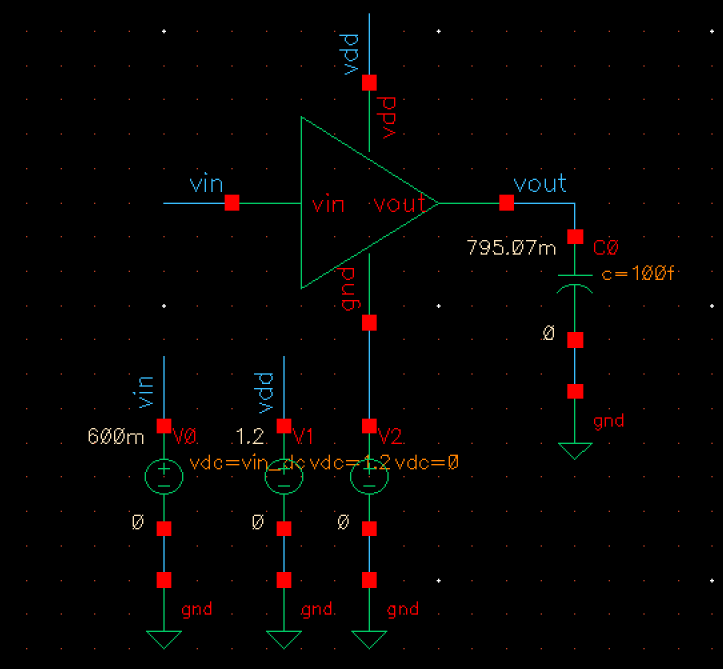
\includegraphics[width=\textwidth]{image-29.png} 
        \caption{Fingers = 2,Finger Width = $1.565\mu$m}
        \label{fig:task9j}
    \end{subfigure}
    % 总图标题
    \label{fig:task9ij}
    \caption{Finger数量影响分析(第一组)}
\end{figure}


\begin{figure}[htbp]
    \centering
    % 第一张子图
    \begin{subfigure}[b]{0.45\textwidth} % 子图宽度为总宽度的45%
        \centering
        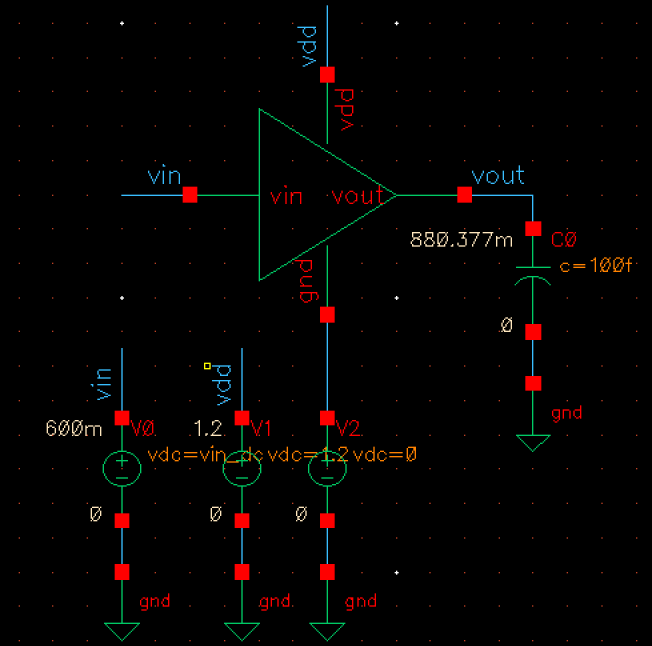
\includegraphics[width=\textwidth]{image-31.png} 
        \caption{Fingers = 3,Finger Width = $1.045\mu$m}
        \label{fig:task9k}
    \end{subfigure}
    \hfill % 添加水平间距
    % 第二张子图
    \begin{subfigure}[b]{0.45\textwidth}
        \centering
        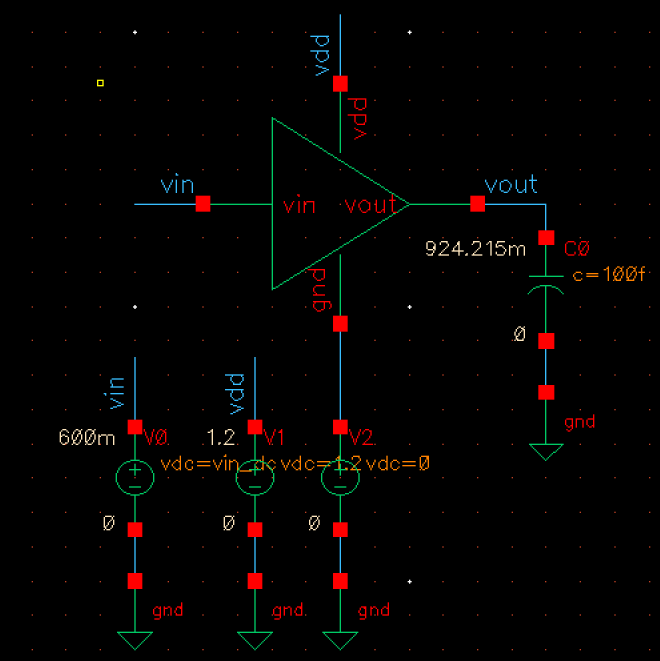
\includegraphics[width=\textwidth]{image-32.png} 
        \caption{Fingers = 4,Finger Width = $780$nm}
        \label{fig:task9l}
    \end{subfigure}
    % 总图标题
    \label{fig:task9kl}
    \caption{Finger数量影响分析(第二组)}
\end{figure}

\begin{figure}[h]
\centering
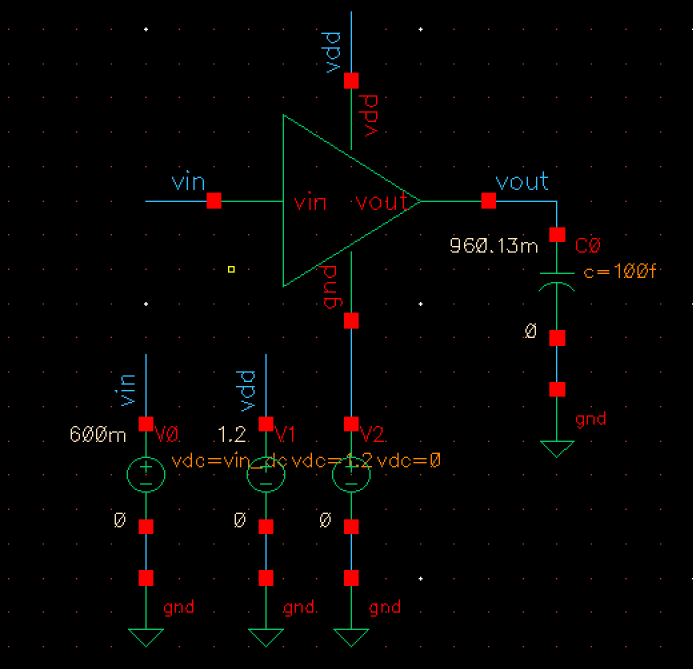
\includegraphics[width=0.7\textwidth]{image-33.png}
\caption{Fingers = 5,Finger Width = $625$nm}
\label{fig:task9m}
\end{figure}

\subsection{理论分析}

\subsubsection{开关阈值的理论计算}
为了使反相器的开关阈值$V_M = V_{DD}/2$,需要满足NMOS和PMOS的跨导参数相等:
\begin{equation}
\beta_n = \beta_p
\end{equation}

即:
\begin{equation}
\mu_n C_{ox}\frac{W_n}{L_n} = \mu_p C_{ox}\frac{W_p}{L_p}
\end{equation}

由于PMOS的载流子迁移率$\mu_p$约为NMOS的$\mu_n$的1/2到1/3,因此需要:
\begin{equation}
\frac{W_p}{W_n} = \frac{\mu_n}{\mu_p} \approx 2 \sim 3
\end{equation}

从实验结果看,当$W_n = 1\mu$m,$W_p = 3.13\mu$m时,比值为3.13,这与理论分析一致。

\subsubsection{Finger结构的影响}
在集成电路版图设计中,晶体管常被分割成多个并联的finger结构:
\begin{equation}
W_{total} = N_{fingers} \times W_{finger}
\end{equation}

使用多finger结构的优点:
\begin{enumerate}
\item \textbf{减小寄生电阻}:多个并联路径降低源漏端的寄生电阻
\item \textbf{改善匹配性}:更规则的版图有利于器件匹配
\item \textbf{提高速度}:减小栅极电阻,提高开关速度
\item \textbf{减小应力效应}:将宽晶体管分成多个窄晶体管可以减小机械应力的影响
\end{enumerate}

从实验结果可以看出,在总宽度固定的情况下,改变finger数量对DC工作点的影响很小,这验证了理论分析。但在高频应用中,多finger结构会表现出更好的性能。





\newpage
\section{任务十:CMOS反相器交直流与时域特性综合分析}

\subsection{任务要求}
\textbf{任务10:在报告中记录三种(DC, AC, TRAN)仿真结果,并对小信号增益和直流偏置情况进行分析。}

\subsection{实验参数}
优化后的CMOS反相器参数:
\begin{itemize}
\item $W_P = 3.13\mu$m,$W_N = 1\mu$m
\item $L_P = L_N = 180$nm
\item 偏置点:$V_{in} = 600$mV
\end{itemize}

\subsection{AC小信号分析}

\subsubsection{幅频响应特性}
图\ref{fig:task10a}展示了在$V_{in} = 600$mV偏置点下的CMOS反相器幅频响应(Bode图)。

\begin{figure}[h]
\centering
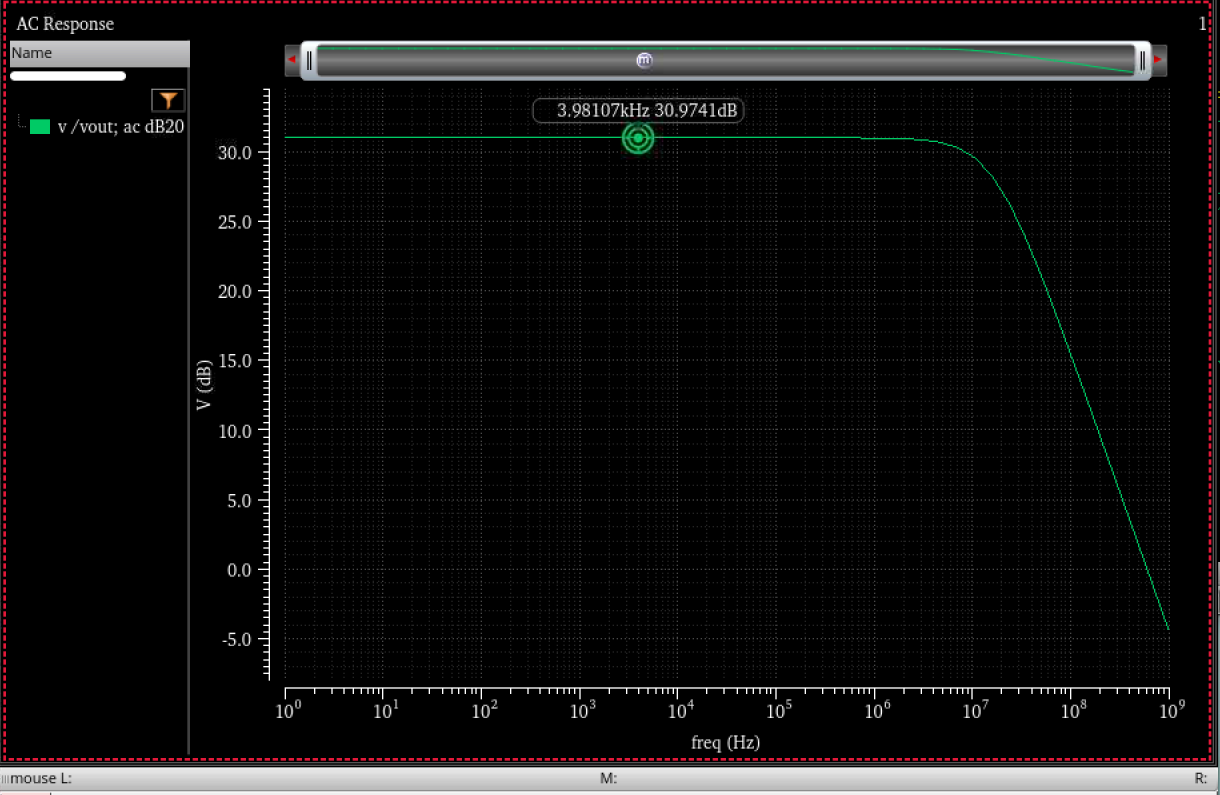
\includegraphics[width=0.8\textwidth]{image-34.png}
\caption{CMOS反相器幅频响应($V_{in} = 600$mV)}
\label{fig:task10a}
\end{figure}

从图中可以读取:
\begin{itemize}
\item 低频增益:$A_v = 30.9741$dB
\end{itemize}

将dB转换为倍数:
\begin{equation}
A_v = 10^{30.9741/20} = 35.37\text{ V/V}
\end{equation}

\subsubsection{DC验证}
为了验证AC仿真的增益,将输入电压从600mV改为599mV,进行DC仿真。图\ref{fig:task10b}展示了DC工作点。

\begin{figure}[h]
\centering
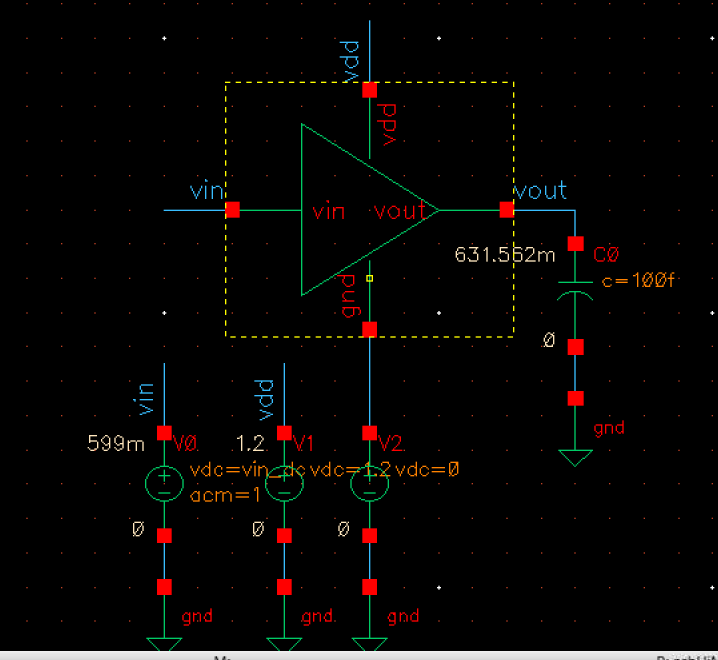
\includegraphics[width=0.7\textwidth]{image-35.png}
\caption{DC工作点验证($V_{in}$从600mV变为599mV)}
\label{fig:task10b}
\end{figure}

从DC仿真结果:
\begin{itemize}
\item 输入电压变化:$\Delta V_{in} = 600\text{mV} - 599\text{mV} = 1\text{mV}$
\item 输出电压变化:$\Delta V_{out} = 631.562\text{mV} - 596.192\text{mV} = 35.37\text{mV}$
\item 计算增益:$A_v = \Delta V_{out}/\Delta V_{in} = 35.37$
\end{itemize}

DC仿真得到的增益35.37倍与AC仿真的30.9741dB(35.37倍)\textbf{完全一致,验证了仿真的正确性。}

\subsubsection{不同偏置点的AC特性}
\textbf{要求分析输入电压为0.4V和0.8V时的增益特性,并思考为什么增益变成负的了。}

\begin{figure}[htbp]
    \centering
    % 第一张子图
    \begin{subfigure}[b]{0.45\textwidth} % 子图宽度为总宽度的45%
        \centering
        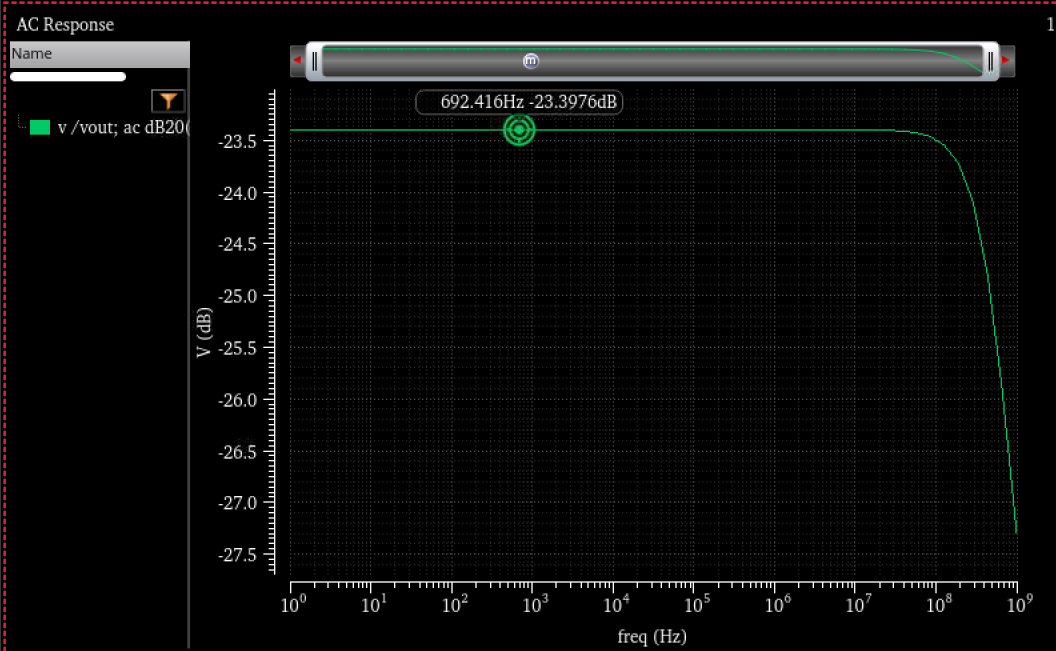
\includegraphics[width=\textwidth]{image-37.png} 
        \caption{CMOS反相器幅频响应($V_{in} = 0.4$V)}
        \label{fig:task10d}
    \end{subfigure}
    \hfill % 添加水平间距
    % 第二张子图
    \begin{subfigure}[b]{0.45\textwidth}
        \centering
        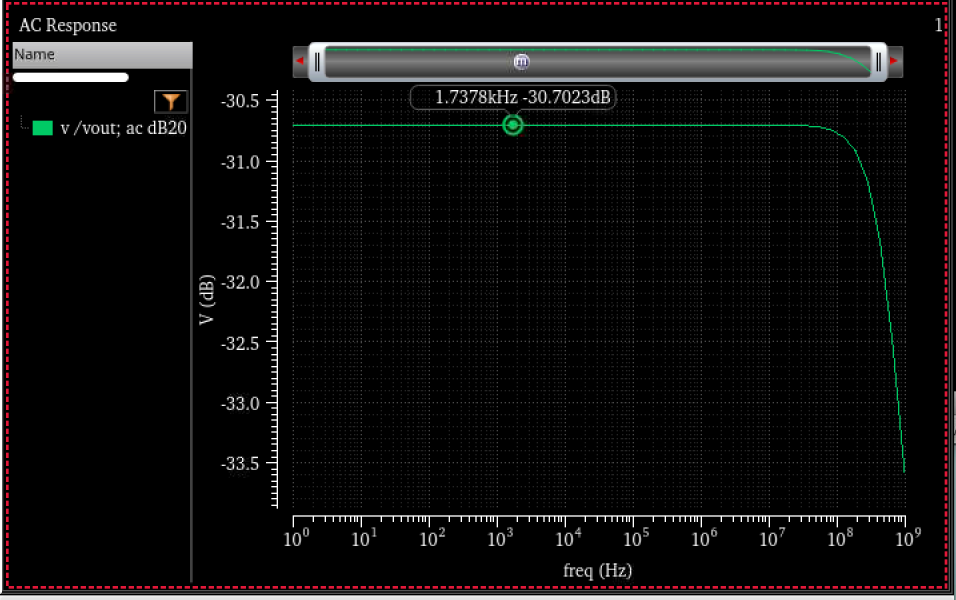
\includegraphics[width=\textwidth]{image-38.png} 
        \caption{CMOS反相器幅频响应($V_{in} = 0.8$V)}
        \label{fig:task10e}
    \end{subfigure}
    % 总图标题
    \label{fig:task10de}
    \caption{Finger数量影响分析(第一组)}
\end{figure}

图\ref{fig:task10d}展示了$V_{in} = 0.4$V时的幅频响应:低频增益:$A_v = -23$dB

图\ref{fig:task10e}展示了$V_{in} = 0.8$V时的幅频响应:低频增益:$A_v = -30$dB

\textbf{为什么增益变成负的了?}

\begin{itemize}
\item 在$V_{in} = 600$mV(接近开关阈值$V_M$)附近,NMOS和PMOS都在饱和区,增益最大
\item 在$V_{in} = 0.4$V或0.8V时,\textbf{偏离最佳工作点,其中一个晶体管进入线性区,增益减小}
\item 负的dB值表示增益小于1(即幅度小于1),这是因为偏离了最佳偏置点,这一点从\ref{fig:task8}的传输特性曲线中也可以看出,当CMOS反相器的工作点偏离$\frac{1}{2}V_{DD}$时,曲线斜率会显著降低,因此增益也会显著下降
\end{itemize}

\subsection{时域瞬态分析(TRAN)}

\subsubsection{小信号时域响应}
\textbf{要求分析时域波形。在偏置点$V_{in} = 600$mV附近叠加小信号,观察输出波形。}

\textbf{信号幅度$A = 100$mV:}

图\ref{fig:task10f}展示了输入和输出的时域波形。

\begin{figure}[h]
\centering
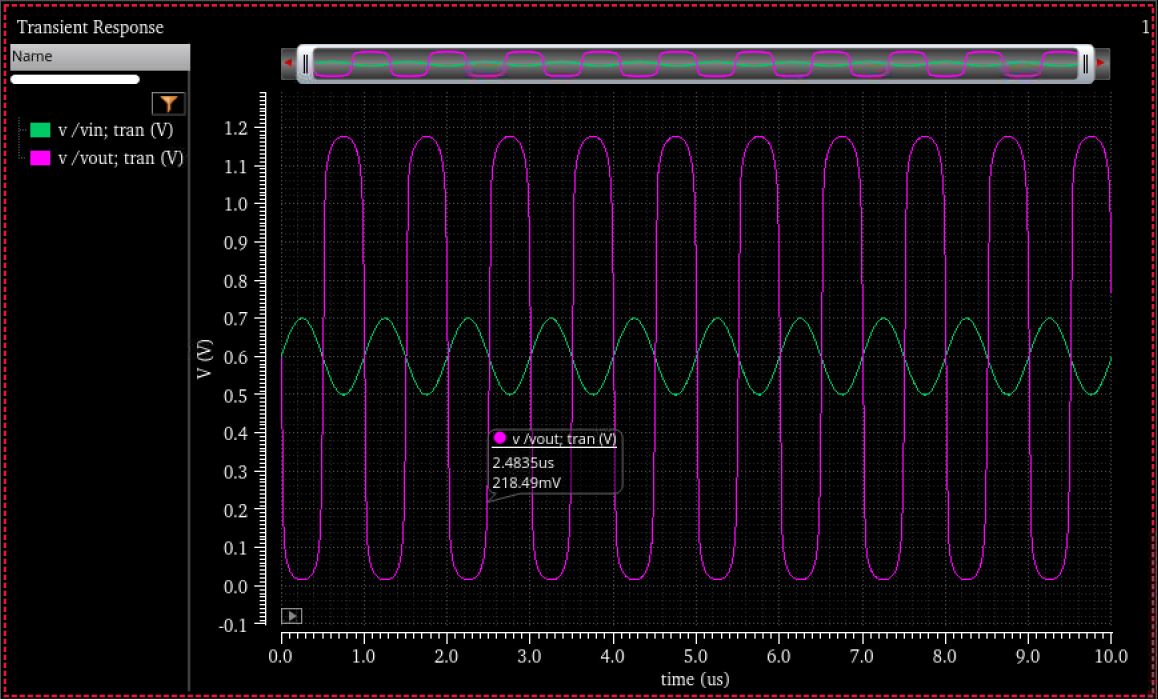
\includegraphics[width=0.8\textwidth]{image-39.png}
\caption{时域响应($V_{in} = 600$mV,$A = 100$mV)}
\label{fig:task10f}
\end{figure}

从波形可以看出:输出信号是输入信号的反相放大版本,在低输入摆幅区域,输出幅度约为输入幅度的35倍(与增益一致)
波形基本保持正弦形状,表明在小信号范围内工作。但是在输入接近波峰的区域,输入电压波形被削平,这是因为此时偏离了线性工作范围,进入了非线性区域,增益与稳定的直流工作点不同。

\textbf{信号幅度$A = 300$mV:}

图\ref{fig:task10g}和图\ref{fig:task10h}展示了较大信号幅度下的时域波形。

\begin{figure}[h]
\centering
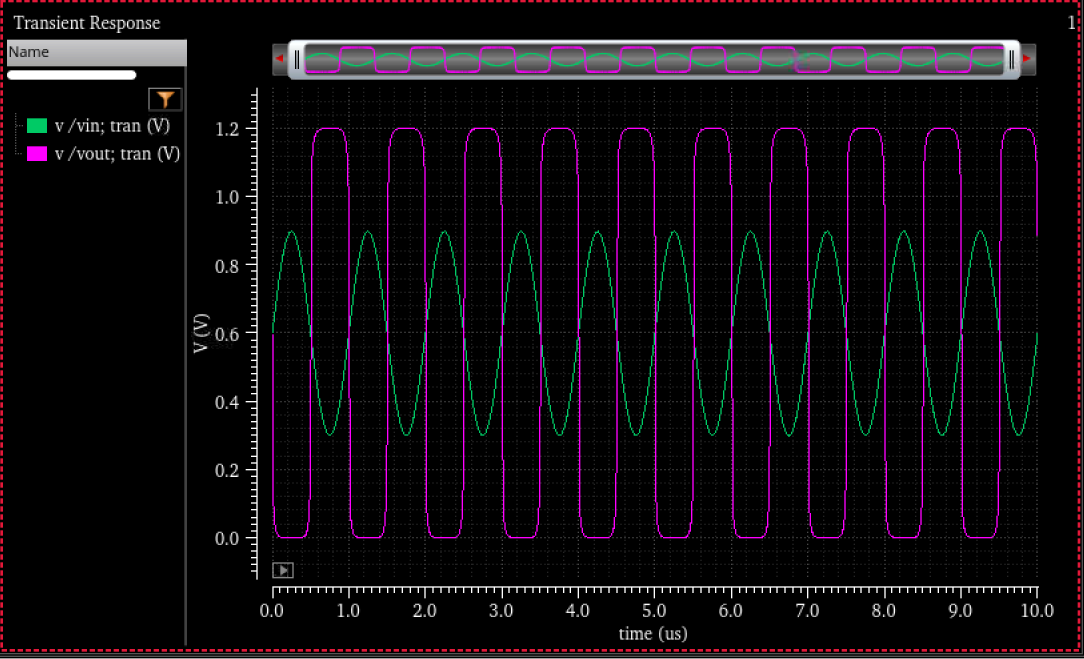
\includegraphics[width=0.8\textwidth]{image-41.png}
\caption{时域响应($V_{in} = 600$mV,$A = 300$mV)- 图1}
\label{fig:task10g}
\end{figure}

\begin{figure}[h]
\centering
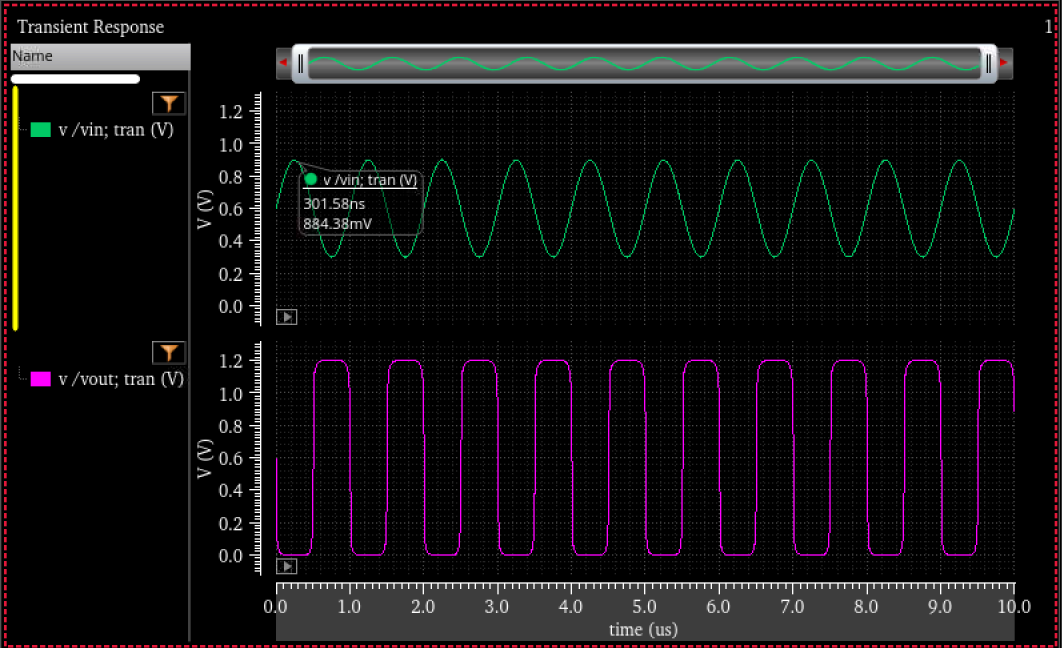
\includegraphics[width=0.8\textwidth]{image-42.png}
\caption{时域响应($V_{in} = 600$mV,$A = 300$mV)- 图2}
\label{fig:task10h}
\end{figure}

从波形可以看出:输入信号幅度增大到300mV后,输入信号范围为300mV到900mV,输出波形出现明显的非线性失真。这是因为输入信号过大,超出了反相器的线性工作范围当输入接近0V或$V_{DD}$时,输出被限制在轨道电压附近


\subsection{综合理论分析}

\subsubsection{小信号增益的理论计算}
CMOS反相器在开关阈值附近工作时,NMOS和PMOS都在饱和区,小信号增益为:
\begin{equation}
A_v = -(g_{mn} + g_{mp})(r_{on} \| r_{op})
\end{equation}

其中:
\begin{itemize}
\item $g_{mn}$,$g_{mp}$分别为NMOS和PMOS的跨导
\item $g_{dsn}$,$g_{dsp}$分别为NMOS和PMOS的输出电导
\item $r_{on} = 1/g_{dsn}$,$r_{op} = 1/g_{dsp}$为输出电阻
\end{itemize}

增益的负号表示反相特性。从实验结果看,增益为35.37,说明:
\begin{equation}
(g_{mn} + g_{mp})(r_{on} \| r_{op}) = 35.37
\end{equation}

\subsubsection{偏置点对增益的影响}
不同偏置点下的增益差异可以用工作区域来解释:

\begin{itemize}
\item \textbf{$V_{in} = 600$mV}(接近$V_M$):
  \begin{itemize}
  \item NMOS和PMOS都在饱和区
  \item 两管的$g_m$都很大,输出电阻也较大
  \item 增益达到最大值
  \end{itemize}

\item \textbf{$V_{in} = 0.4$V}(较低):
  \begin{itemize}
  \item NMOS刚进入饱和区,$g_{mn}$较小
  \item PMOS在线性区,$r_{op}$很小
  \item 总体增益很小(小于1)
  \end{itemize}

\item \textbf{$V_{in} = 0.8$V}(较高):
  \begin{itemize}
  \item NMOS在线性区,$r_{on}$很小
  \item PMOS刚进入饱和区,$g_{mp}$较小
  \item 总体增益很小(小于1)
  \end{itemize}
\end{itemize}

\subsubsection{小信号条件与大信号失真}
小信号分析的前提是信号幅度足够小,使得晶体管参数($g_m$,$r_o$等)可以近似为常数。从实验可以看出:
\begin{itemize}
\item 当$A = 100$mV时,输入信号范围为500mV到700mV,输出基本保持线性
\item 当$A = 300$mV时,输入信号范围为300mV到900mV,输出出现削波失真
\end{itemize}

失真的原因是:
\begin{itemize}
\item 当$V_{in}$过低时,NMOS接近截止,输出被拉高到接近$V_{DD}$
\item 当$V_{in}$过高时,PMOS接近截止,输出被拉低到接近0V
\item 这种削波限制了反相器作为线性放大器的动态范围
\end{itemize}

\subsubsection{三种仿真方法的关系}
\begin{itemize}
\item \textbf{DC仿真}:确定静态工作点,计算偏置电压和电流
\item \textbf{AC仿真}:在工作点处线性化,分析小信号频率响应和增益
\item \textbf{TRAN仿真}:完整的非线性时域分析,可以观察大信号行为和失真,并且可以揭示AC分析无法捕捉的非线性效应
\end{itemize}



\end{document}
